\documentclass{report}

\usepackage[colorlinks=true, pdfstartview=FitV, linkcolor=xkcdBlue, citecolor=xkcdRed, urlcolor=xkcdGreen]{hyperref}
\usepackage{graphicx}
\usepackage{color}
\usepackage{amsmath}
\usepackage{hyperref}
\usepackage{enumerate}
\usepackage{xcolor}
\usepackage{xkcdcolors}
\usepackage[]{algorithm2e}
\usepackage{float}
\usepackage{listings}
\usepackage{xcolor}

\lstset{
    language=Python,
    basicstyle=\ttfamily\small,
    keywordstyle=\color{blue},
    commentstyle=\color{gray},
    stringstyle=\color{red},
    breaklines=true
}


% \addtolength{\topmargin}{-.7in}
% \addtolength{\textheight}{.6in}
\usepackage[a4paper, left=1.80cm, right=1.80cm, top=2cm, bottom=2cm, bindingoffset=0cm]{geometry} 


\begin{document}


\Large
\textbf{AE4868-II (2025/2026) - Assignment 3} \\
\normalsize \\

Name: Ismael Gallo López \\

Student number: 6541356 \\

Github link: \textit{\href{https://github.com/ismaelgallolopez/numerical-astrodynamics-GALLO_LOPEZ_Ismael}{\nolinkurl{https://github.com/ismaelgallolopez/numerical-astrodynamics-GALLO_LOPEZ_Ismael}}} \\

Time spent per exercise:
\begin{enumerate}
    \item 6h
    \item 4h
    \item 4h
    \item 4h
    \item 3h

\end{enumerate} 

People you worked with (if none, state this):

\begin{itemize}
    \item Daniel Pérez Trias
    \item Gonzalo Guerrero Rodríguez 
    \item Andreu Craus Vidal
    \item Gemini 3
\end{itemize}

\clearpage

% \noindent\textit{Use this \LaTeX~file as a template for your report. All text that is not italic should be kept. All text that is italic, and all \ldots~should be removed and replaced by your answers. Only text that replaces \textbf{bold text} counts towards your line limit.}
% KC: bold text here > bold text?

\section*{Question 1}

\subsection*{a}

\begin{figure}[H]
    \centering
    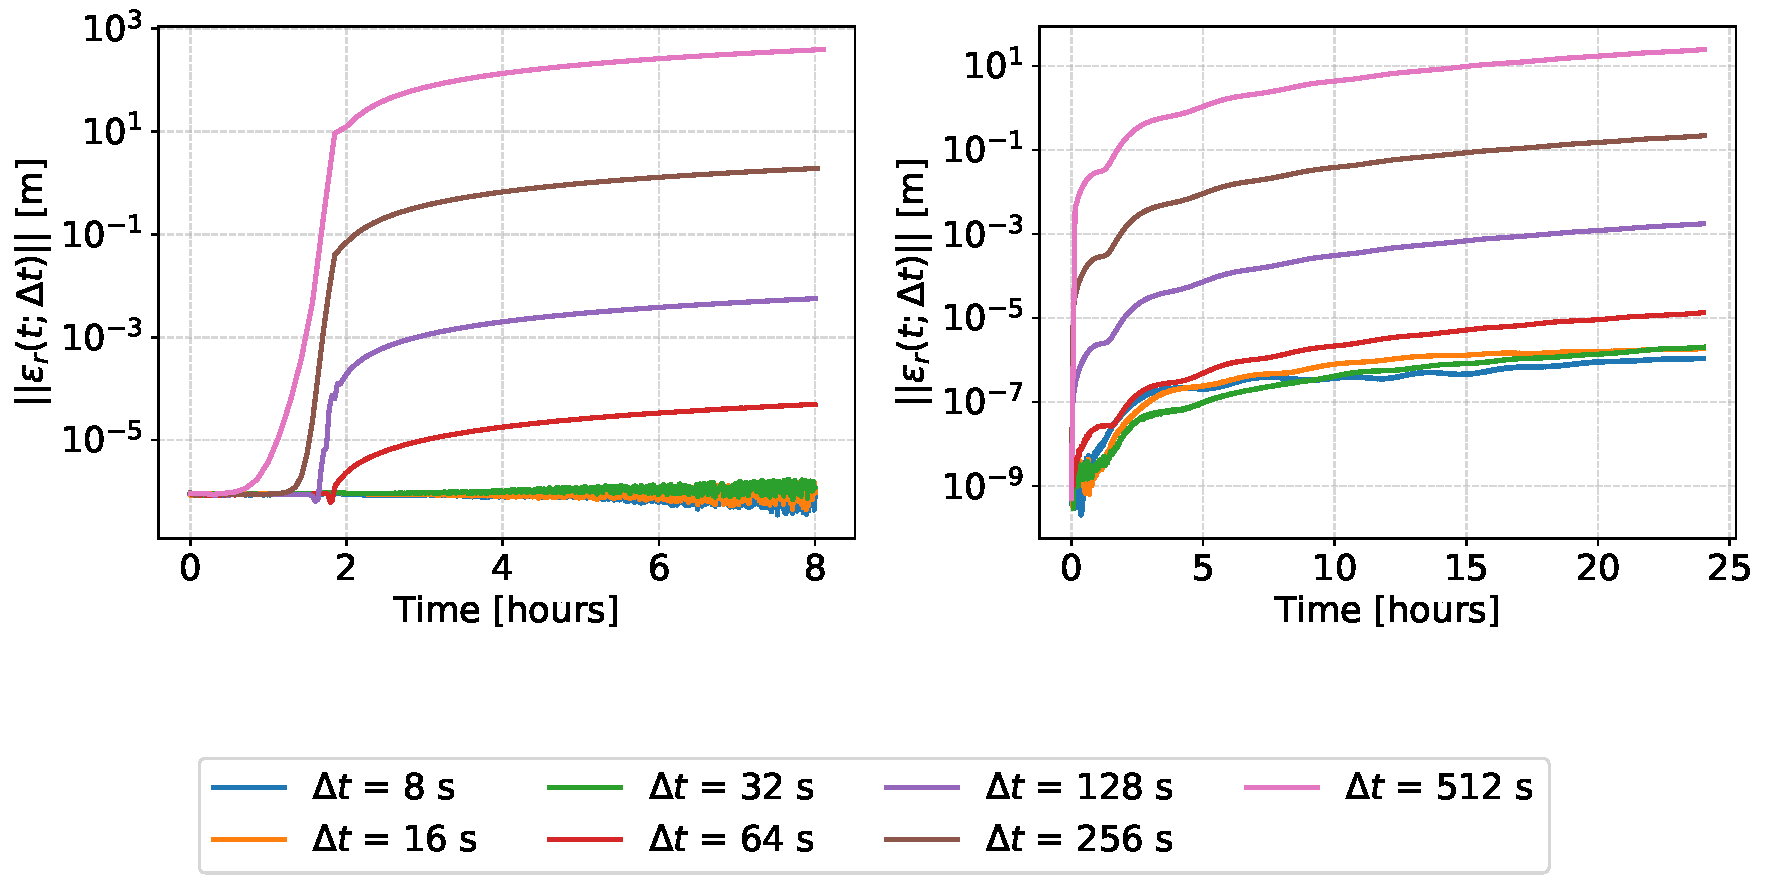
\includegraphics[width=0.8\textwidth]{../../figures/Q1_error_vs_time_combined.pdf}
    \caption{Integration error as a function of time for both the Flyby and GCO500 phases, for the different time steps.}
    \label{fig:Q1_error_vs_time_combined}
\end{figure}

\subsection*{b}

\begin{figure}[H]
    \centering
    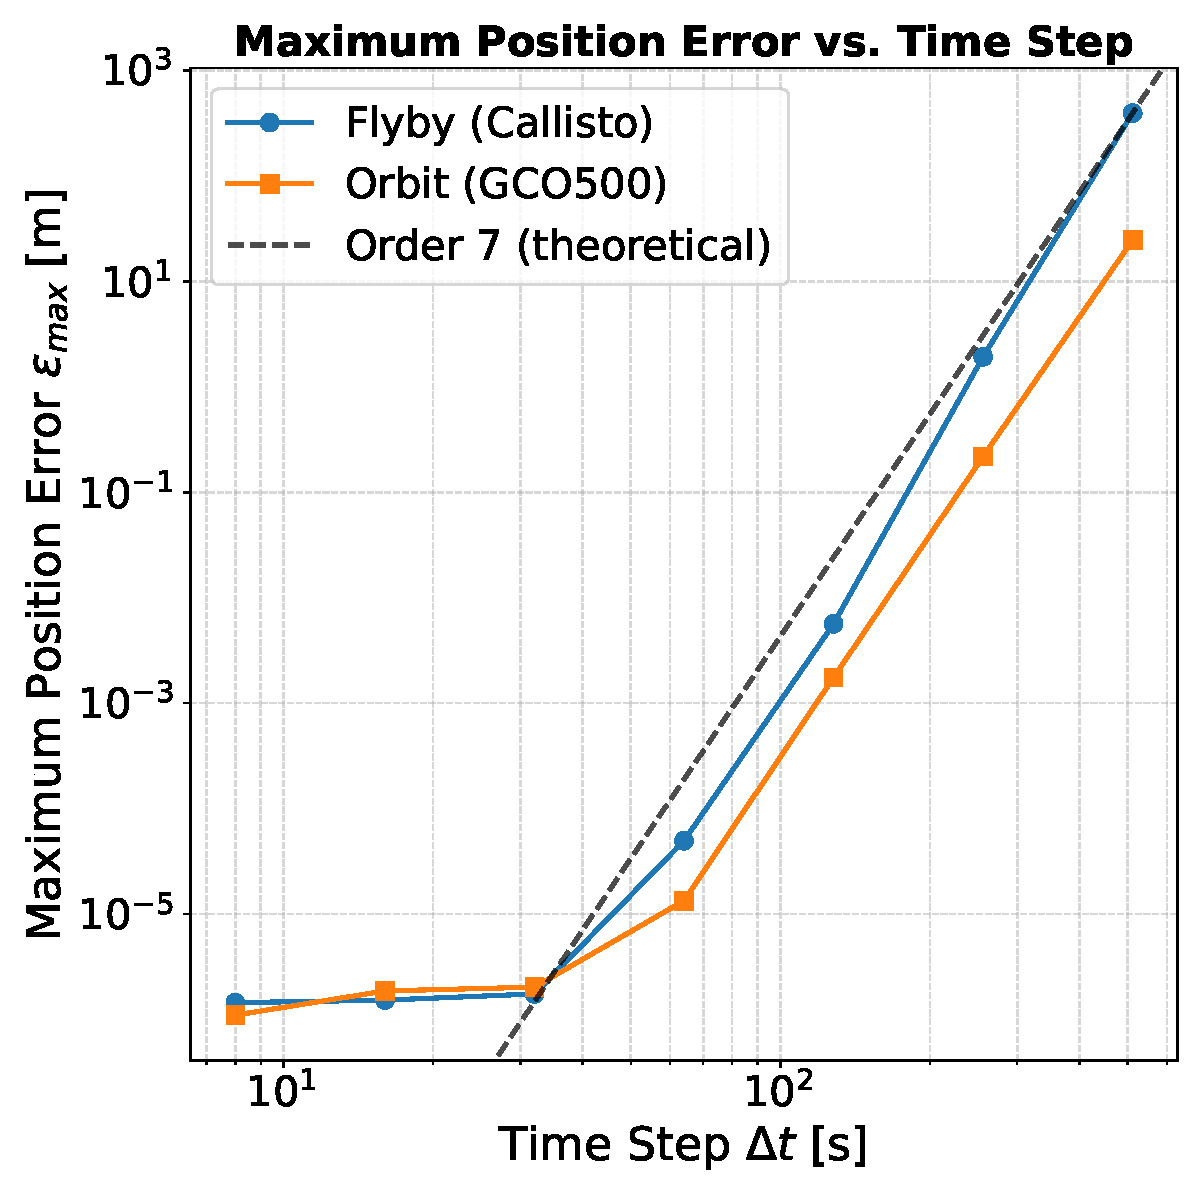
\includegraphics[width=0.7\textwidth]{../../figures/Q1_max_error_vs_timestep.pdf}
    \caption{Maximum error as a function of time step for the GCO500 and flyby phases.}
    \label{fig:Q1_max_error_vs_timestep}
\end{figure}

\subsection*{c}

\begin{enumerate}[i.]
    \item Mathematical equation that describes behavior in maximum truncation error with time step:

    \begin{equation} \label{eq:trunc_error_RK}
        \epsilon_{max}(\Delta t) \approx K (\Delta t)^N
    \end{equation}

    where $K$ is a constant and $N$ is the order of the integrator, $N=7$ for RKF7(8) with fixed step size.

    \item Range of time steps where truncation error is dominant (GCO500): $\Delta t \in \{64, 128, 256, 512 \} \mathrm{ s}$ 

    \item Range of time steps where truncation error is dominant (flyby): $\Delta t \in \{32, 64, 128, 256, 512 \} \mathrm{ s}$

    \item From the error behaviour in Fig.~\ref{fig:Q1_error_vs_time_combined}, it can be inferred that the maximum error is driven by the truncation error, at least, for $\Delta t \geq 64 \mathrm{ s}$. 
    To confirm this, and to analyze the limit case observed in Fig.~\ref{fig:Q1_max_error_vs_timestep}, the integration error is plotted only for $\Delta t \in \{32, 16, 8\} \mathrm{ s}$ in Fig.~\ref{fig:Q1_error_vs_time_low_timesteps}. 
    From the quasi-random evolution for all the timesteps plotted for the flyby it can be stated that the dominant error source is not truncation error. 
    On the other hand, for the GCO500 integration, the $\Delta t = 32 \mathrm{ s}$ case shows a behavior consistent with the truncation error model (Eq.~\ref{eq:trunc_error_RK}).
    However, even thought the $\Delta t = 16 \mathrm{ s}$ and $\Delta t = 8 \mathrm{ s}$ cases show a similar behaviour, the error magnitude should be much smaller if it were truncation-driven, so it can be inferred that the dominant error source is rounding error.
\end{enumerate}

\begin{figure}
    \centering
    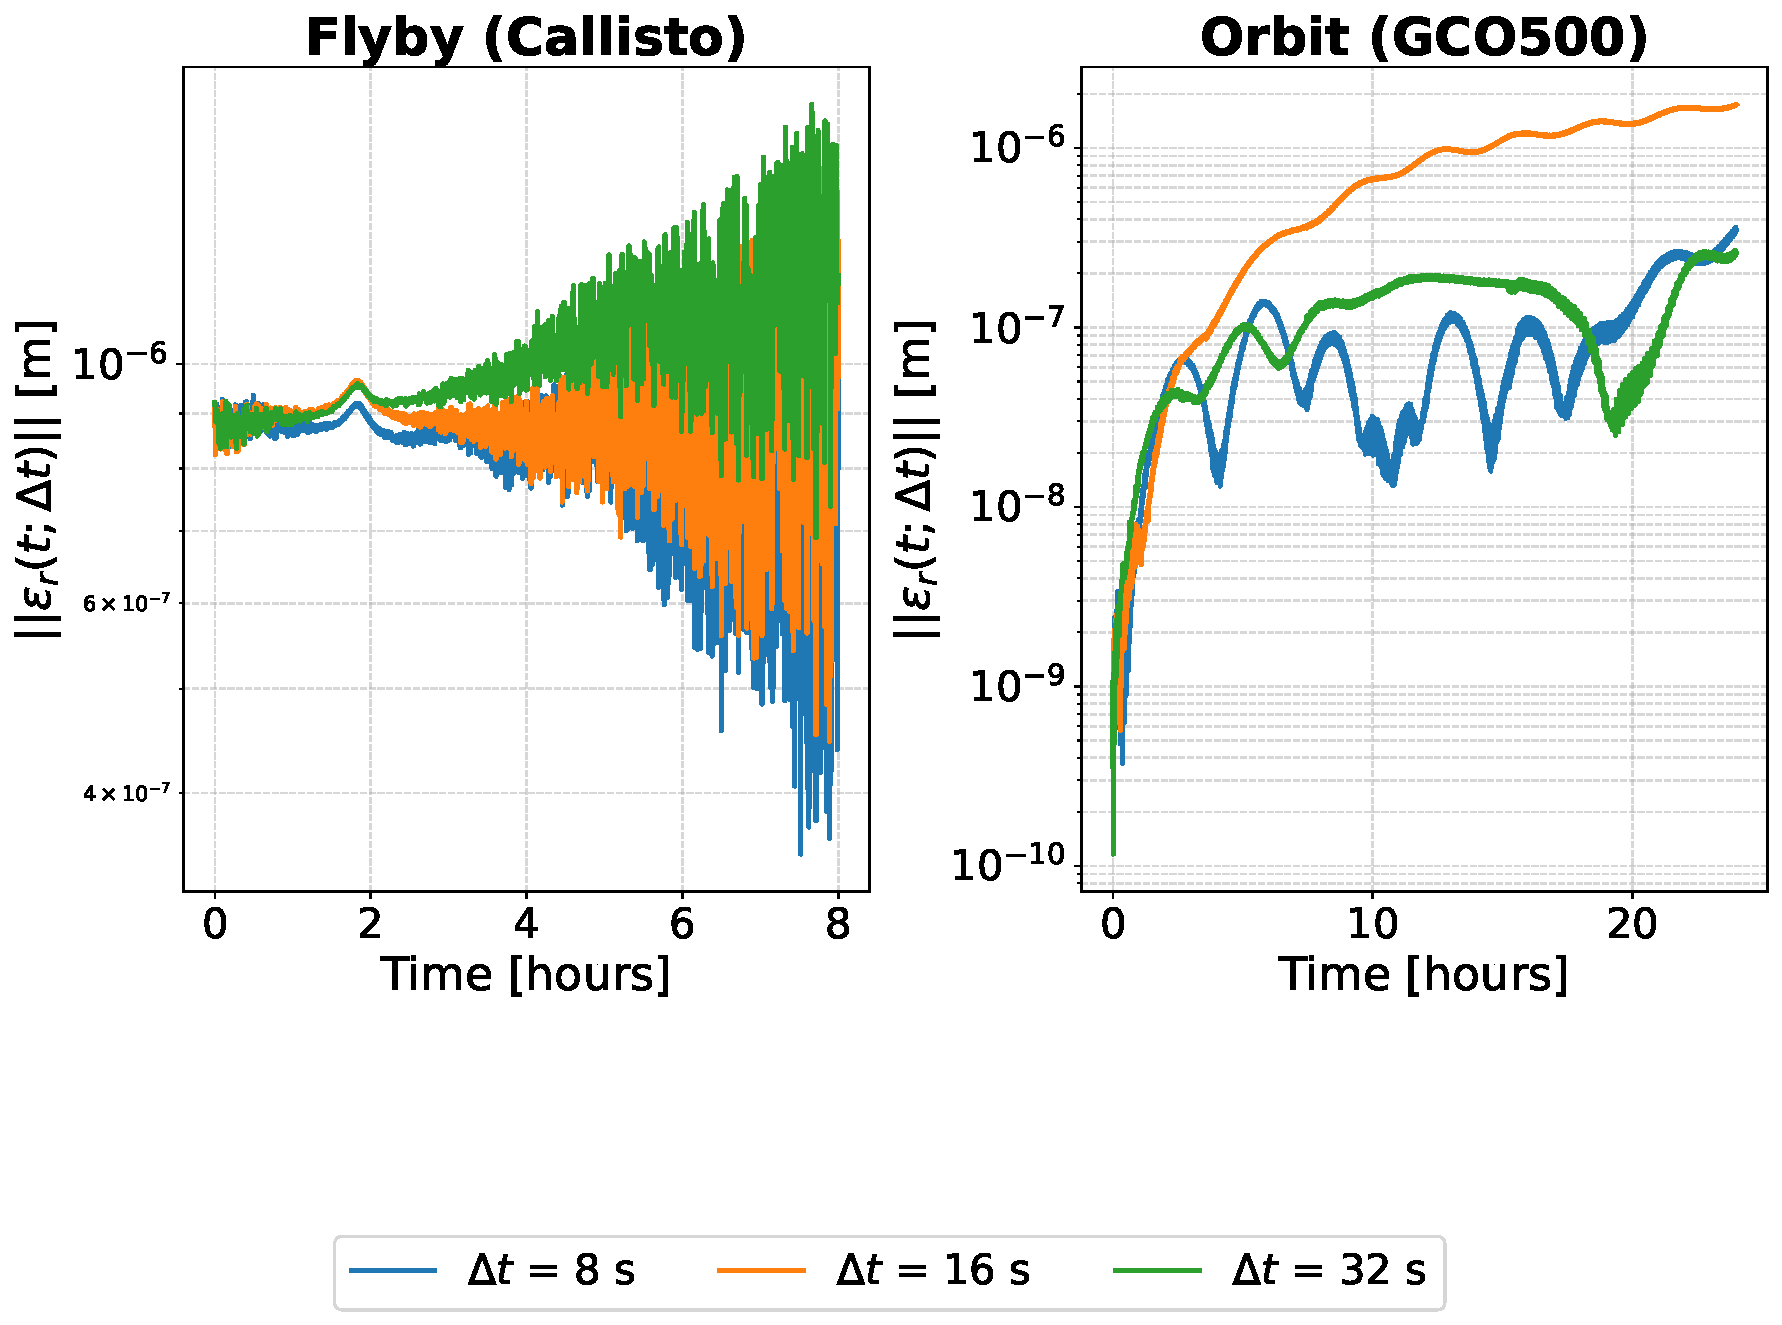
\includegraphics[width=0.7\textwidth]{../../figures/Q1_error_vs_time_low_timesteps.pdf}
    \caption{Integration error as a function of time for both the Flyby and GCO500 phases, only for the 3 smallest time steps.}
    \label{fig:Q1_error_vs_time_low_timesteps}
\end{figure}

\clearpage

\section*{Question 2}

\subsection*{a}

\begin{figure}[H]
    \centering
    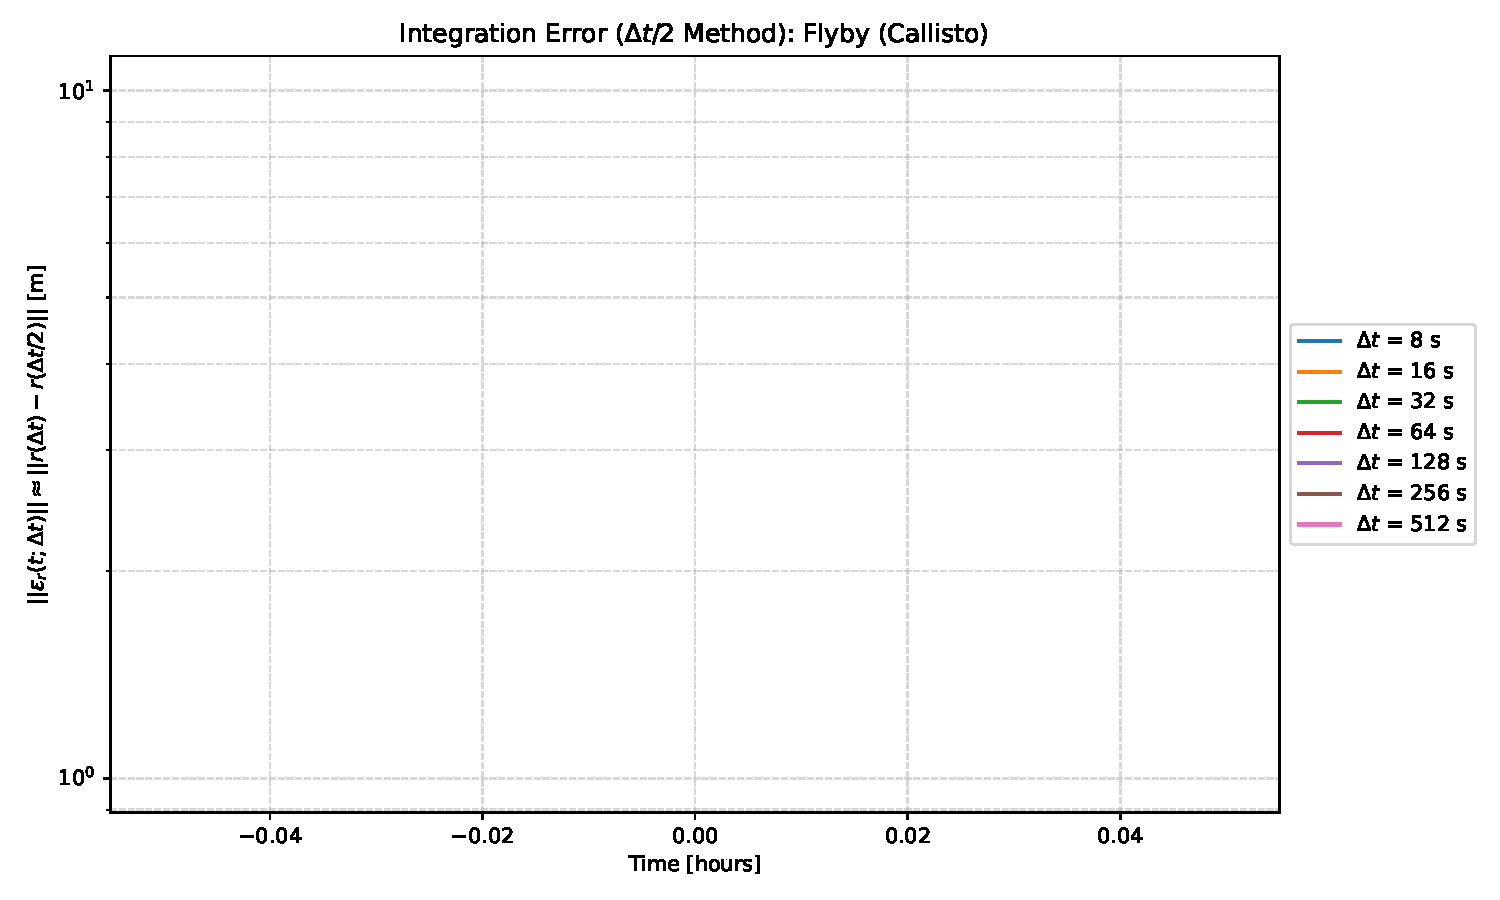
\includegraphics[width=0.7\textwidth]{../../figures/Q2a_error_vs_time_flyby.pdf}
    \caption{Integration error as a function of time for both the Flyby phase, computed as $\mbox{\(\epsilon (t; \Delta t) \approx \mathbf{r} (t; \Delta t) - \mathbf{r} (t; \Delta t/2)\)}$.}
    \label{fig:Q2a_error_vs_time_flyby}
\end{figure}

\begin{figure}[H]
    \centering
    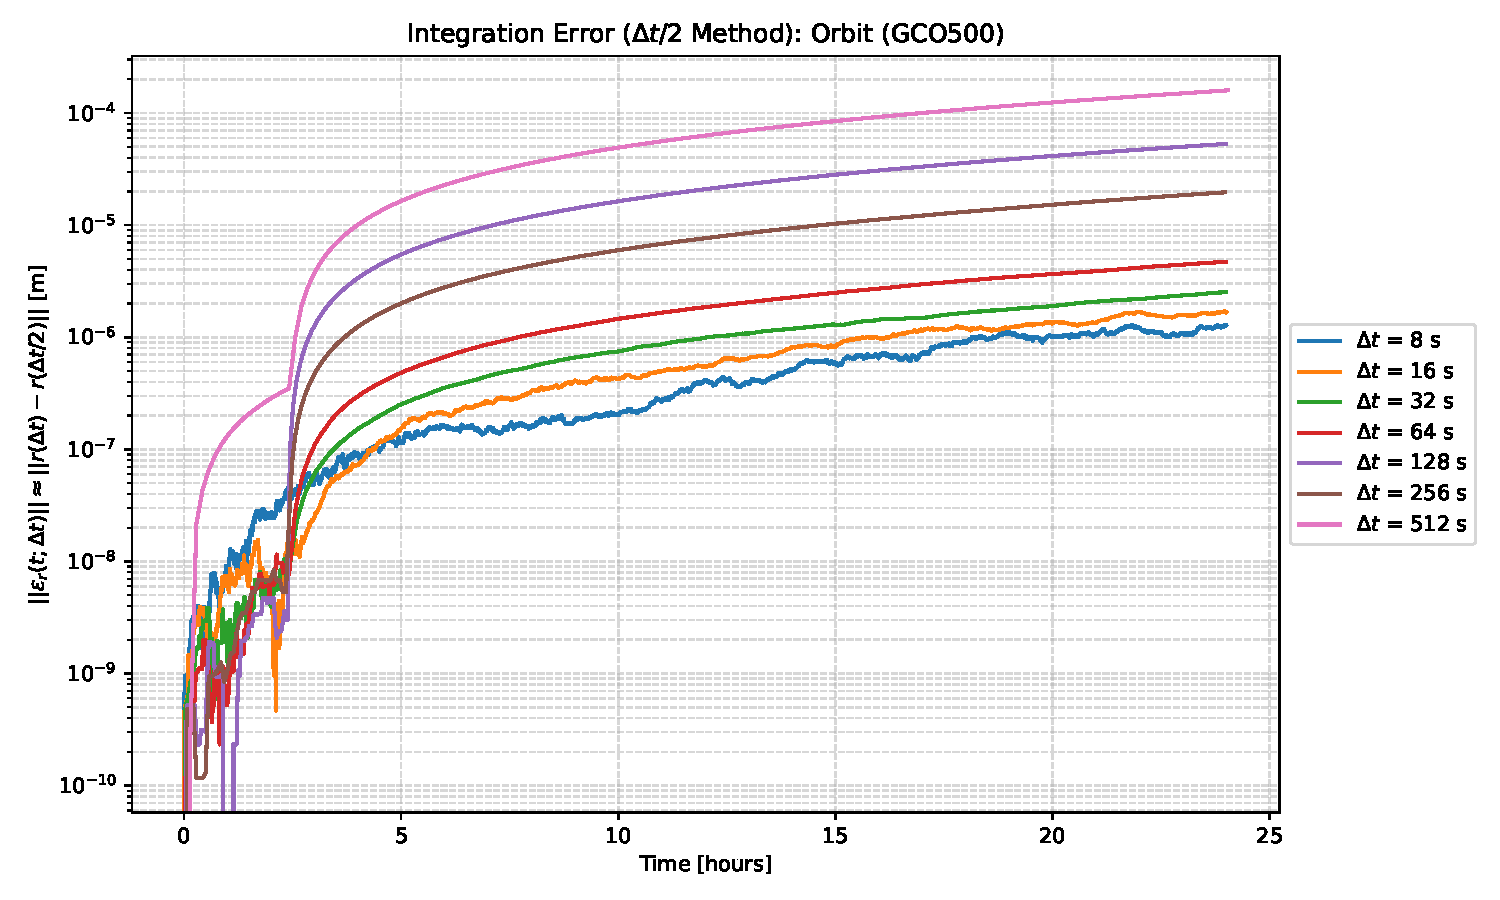
\includegraphics[width=0.7\textwidth]{../../figures/Q2a_error_vs_time_orbit.pdf}
    \caption{Integration error as a function of time for both the GCO500 phase, computed as $\mbox{\(\epsilon (t; \Delta t) \approx \mathbf{r} (t; \Delta t) - \mathbf{r} (t; \Delta t/2)\)}$.}
    \label{fig:Q2a_error_vs_time_orbit}
\end{figure}

Mathematical assumption behind error quantification: 

\begin{equation}
    \mathbf{r}_{true} \approx \mathbf{r}(t; \Delta t) + C (\Delta t)^{p+1},
\end{equation} \label{eq:half_step_error_assumption}

which implies that the dominant error term is the truncation error, and that the error can be approximated by the difference between two solutions with different time steps. 
Hence, the error of the solution with the bigger time step is much bigger than the error of the solution with the smaller time step.

\subsection*{b}

\begin{figure}[H]
    \centering
    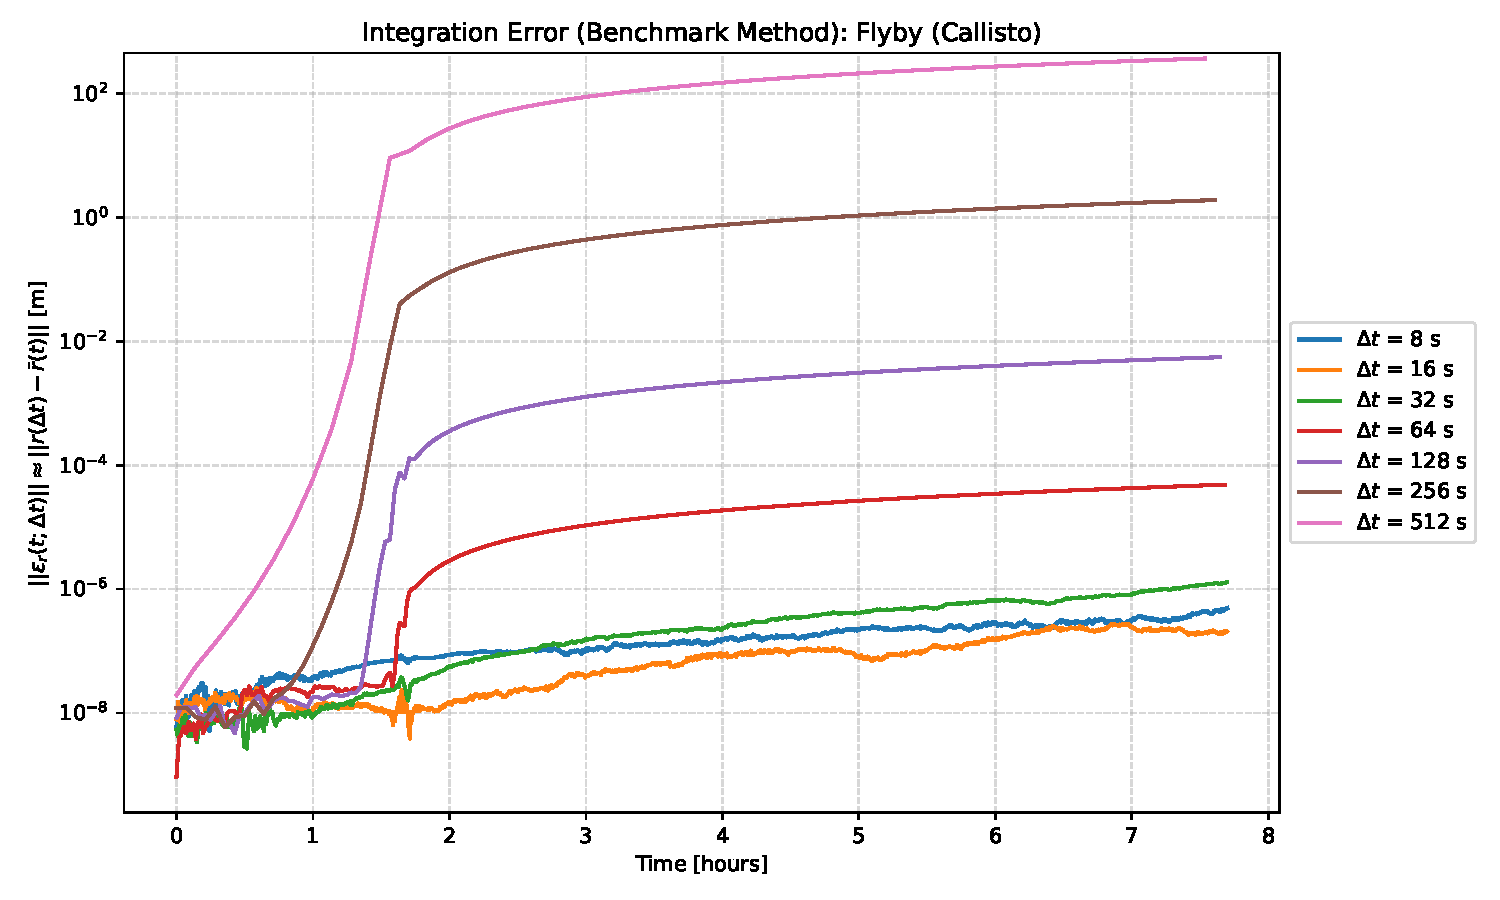
\includegraphics[width=0.7\textwidth]{../../figures/Q2b_error_vs_time_flyby.pdf}
    \caption{Integration error as a function of time for the Flyby phase, computed as $\mbox{\(\epsilon (t; \Delta t) \approx \mathbf{r} (t; \Delta t) - \mathbf{\overline{r}} (t)\)}$.}
    \label{fig:Q2b_error_vs_time_flyby}
\end{figure}

\begin{figure}[H]
    \centering
    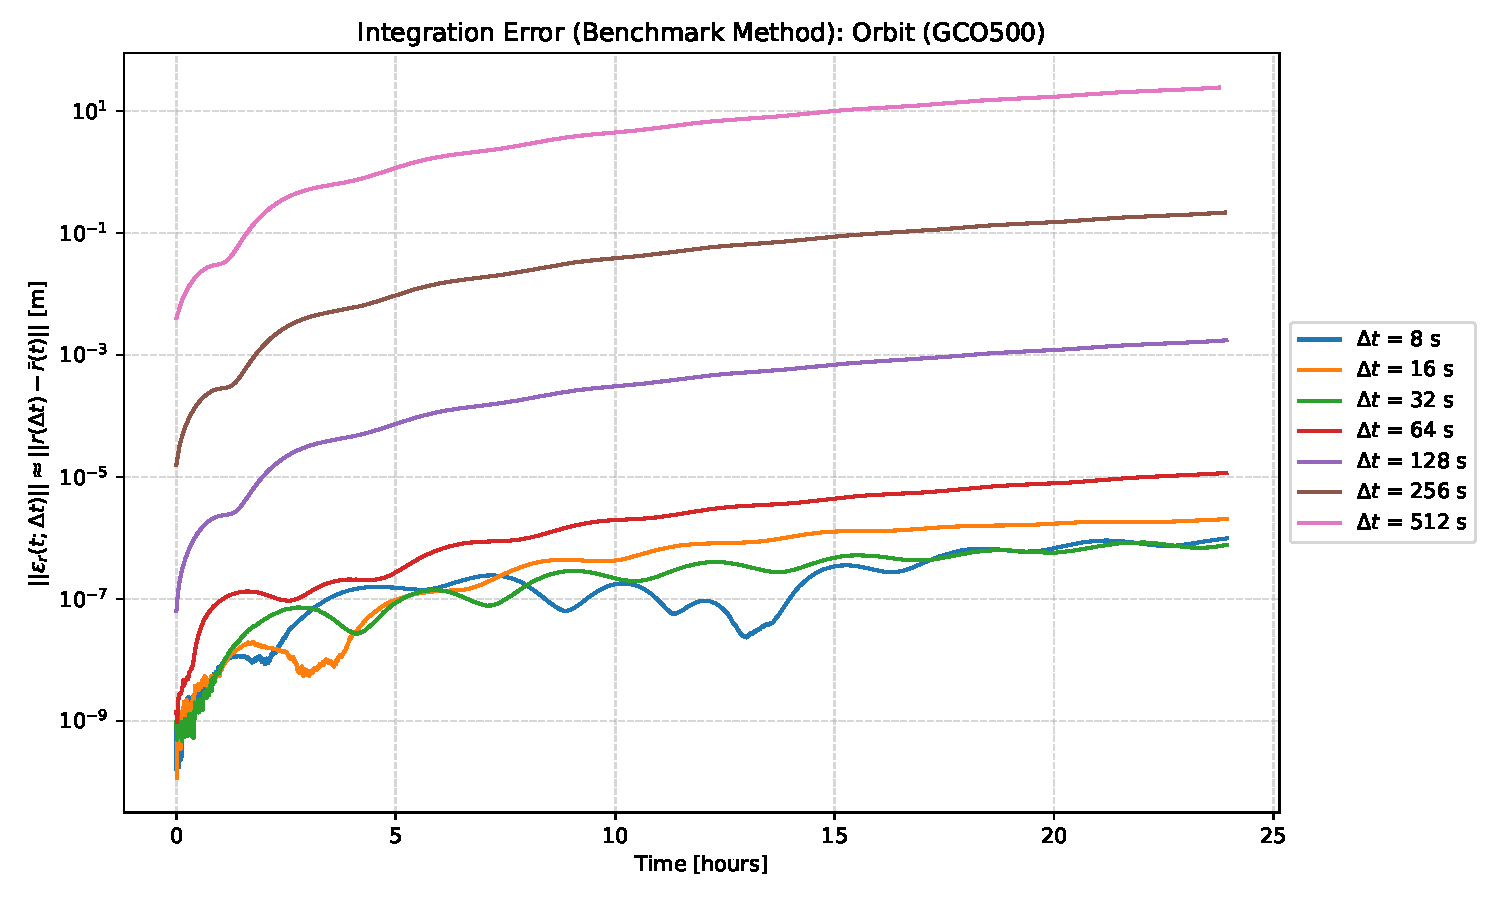
\includegraphics[width=0.7\textwidth]{../../figures/Q2b_error_vs_time_orbit.pdf}
    \caption{Integration error as a function of time for the GCO500 phase, computed as $\mbox{\(\epsilon (t; \Delta t) \approx \mathbf{r} (t; \Delta t) - \mathbf{\overline{r}} (t)\)}$.}
    \label{fig:Q2b_error_vs_time_orbit}
\end{figure}

Mathematical assumption behind error quantification: the benchmark solution $\mathbf{\overline{r}} (t)$ is sufficiently accurate such that the error of the solution with time step $\Delta t$ can be approximated by the difference between the solution and the benchmark, or the interpolated benchmark if no data is available at that epoch.

\subsection*{c}

\begin{figure}[H]
    \centering
    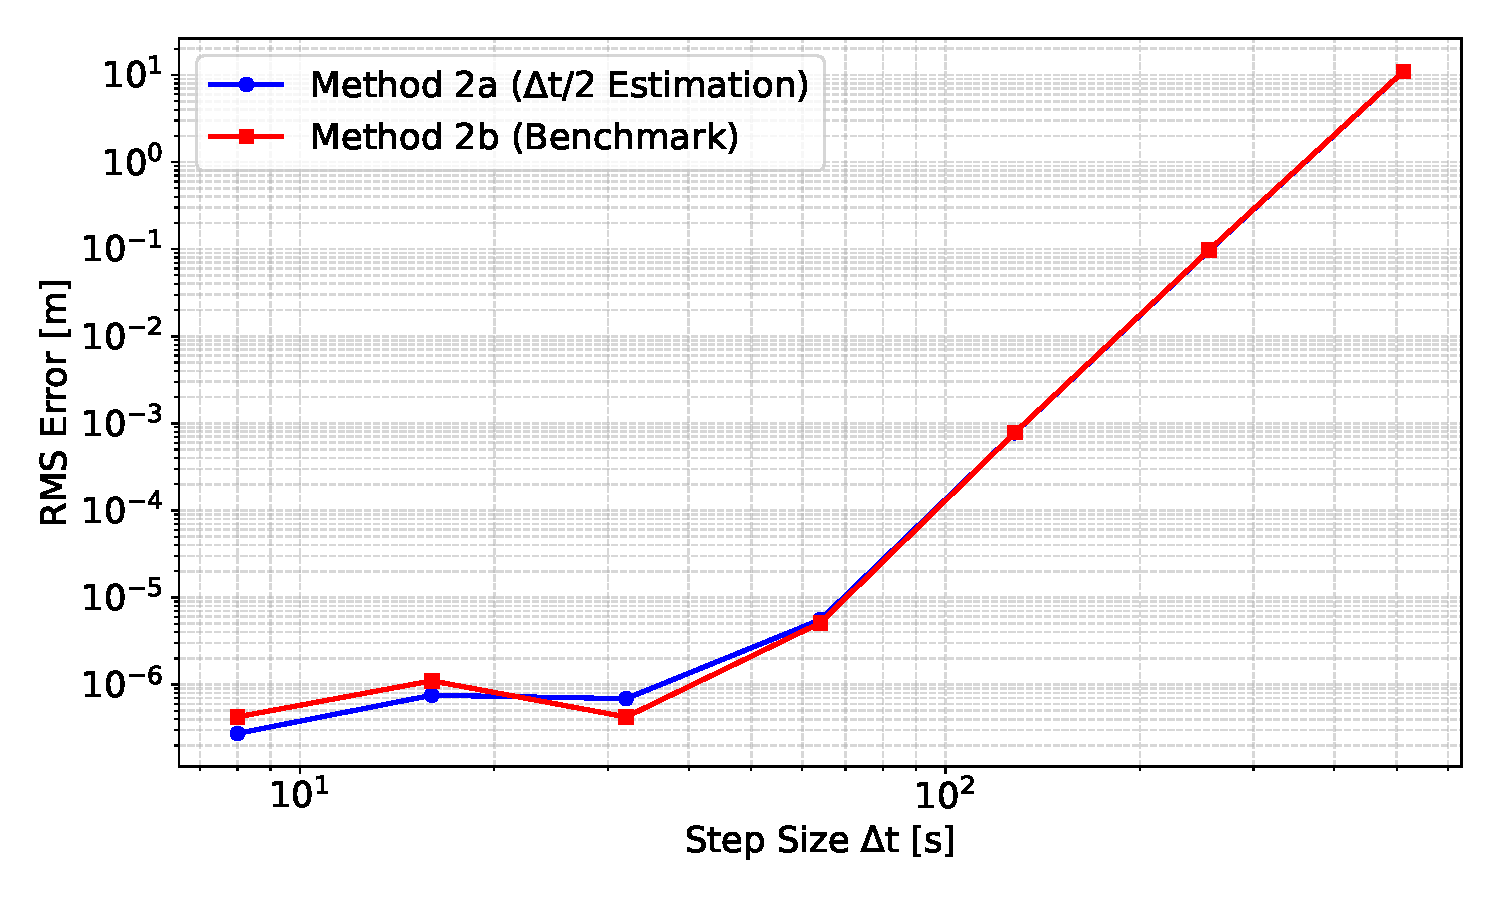
\includegraphics[width=0.7\textwidth]{../../figures/Q2c_convergence_orbit.pdf}
    \caption{Maximum integration error as a function of time step for the GCO500 phase, for the 2 definitions used.}
    \label{fig:Q2c_convergence_orbit}
\end{figure}

\begin{figure}[H]
    \centering
    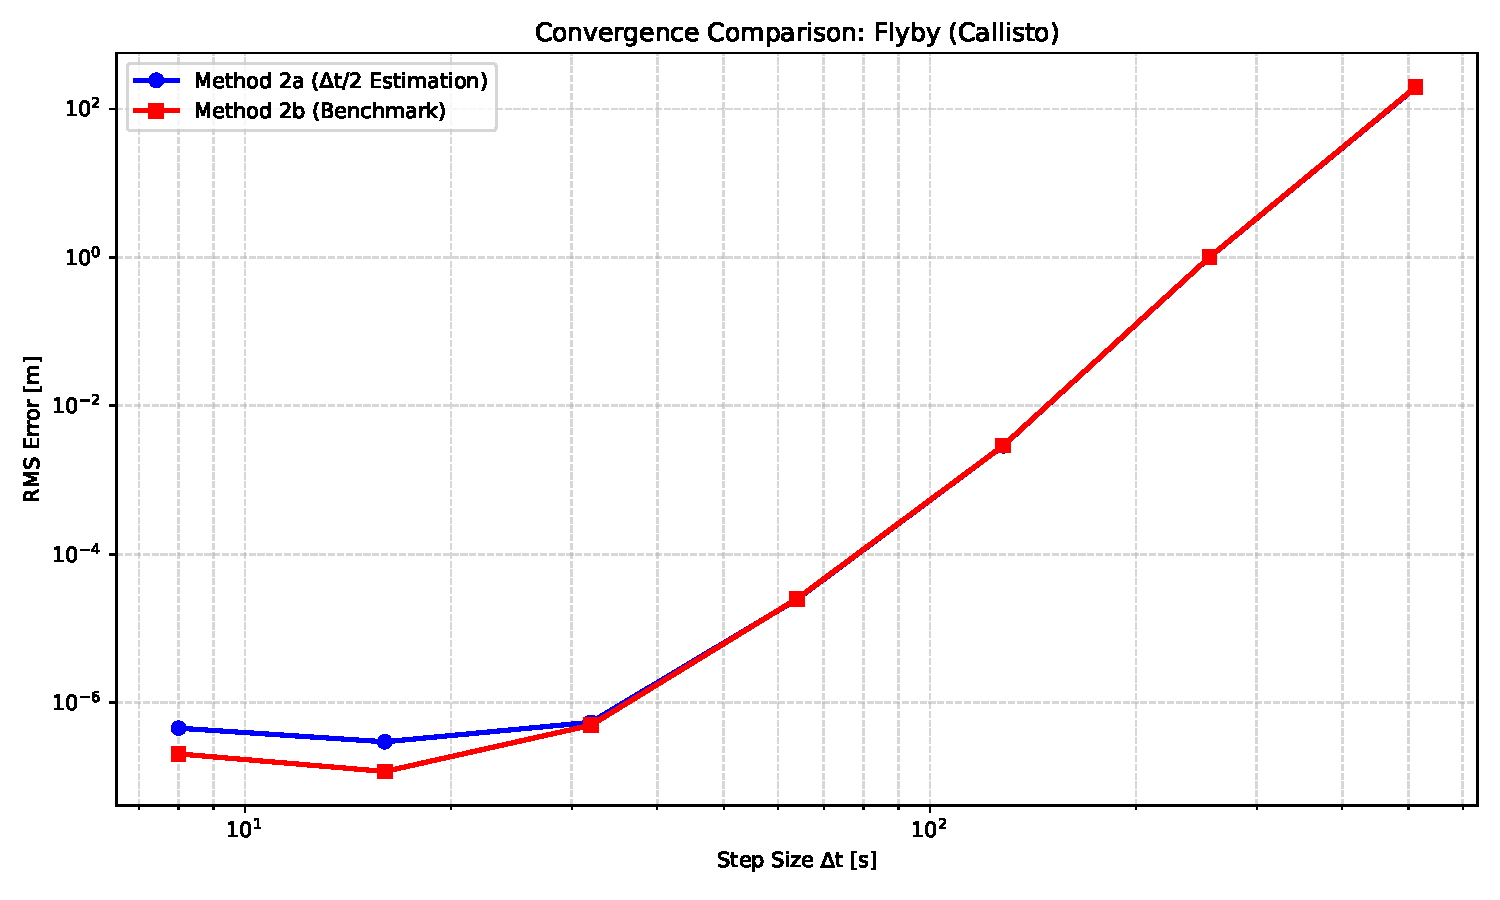
\includegraphics[width=0.7\textwidth]{../../figures/Q2c_convergence_flyby.pdf}
    \caption{Maximum integration error as a function of time step for the Flyby phase, for the 2 definitions used.}
    \label{fig:Q2c_convergence_flyby}
\end{figure}

Range of time steps where results match reasonably well between questions (a) and (b), per phase (see \autoref{fig:Q2c_convergence_orbit} and \autoref{fig:Q2c_convergence_flyby}): 

\begin{itemize}
    \item GCO500: $\Delta t \geq 64 \mathrm{ s}$
    \item Flyby: $\Delta t \geq 32 \mathrm{ s}$
    \end{itemize}

Range of time steps where results do not match reasonably well between questions (a) and (b), per phase (see \autoref{fig:Q2c_convergence_orbit} and \autoref{fig:Q2c_convergence_flyby}): 

\begin{itemize}
    \item GCO500: $\Delta t < 64 \mathrm{ s}$
    \item Flyby: $\Delta t < 32 \mathrm{ s}$
    \end{itemize}

Most of the examples fall under the assumption that the dominant source of error is the truncation error.
However, for the smallest time steps, the error is not dominated by the truncation error, and the assumptions behind both error quantification methods do not hold, so the differences between the quantification method has a quasi-random nature, hence introducing changes between both methods.

\subsection*{d}
For the time steps where truncation error is dominant, do the error estimates obtained in questions 1 and 2b correspond well: \textbf{yes}.

% \textbf{\textit{Explain the underlying reasons why the two do (not) correspond well to one another.}}
Since the truncation error is dominant, the error decreases proportionall to $\Delta t^7$ for the method used, so a halving of the time step should lead to a decrease in error by a factor of 128.
Hence, subtracting two solutions with time steps $\Delta t$ and $\Delta t/2$ should give an error estimate that is close to the error of the solution with time step $\Delta t$ .
Same reasoning applies to the benchmark method, where the time step difference are even more pronounced (for the truncation-driven regime).

\clearpage
\section*{Question 3}
\subsection*{a}

\begin{figure}[H]
    \centering
    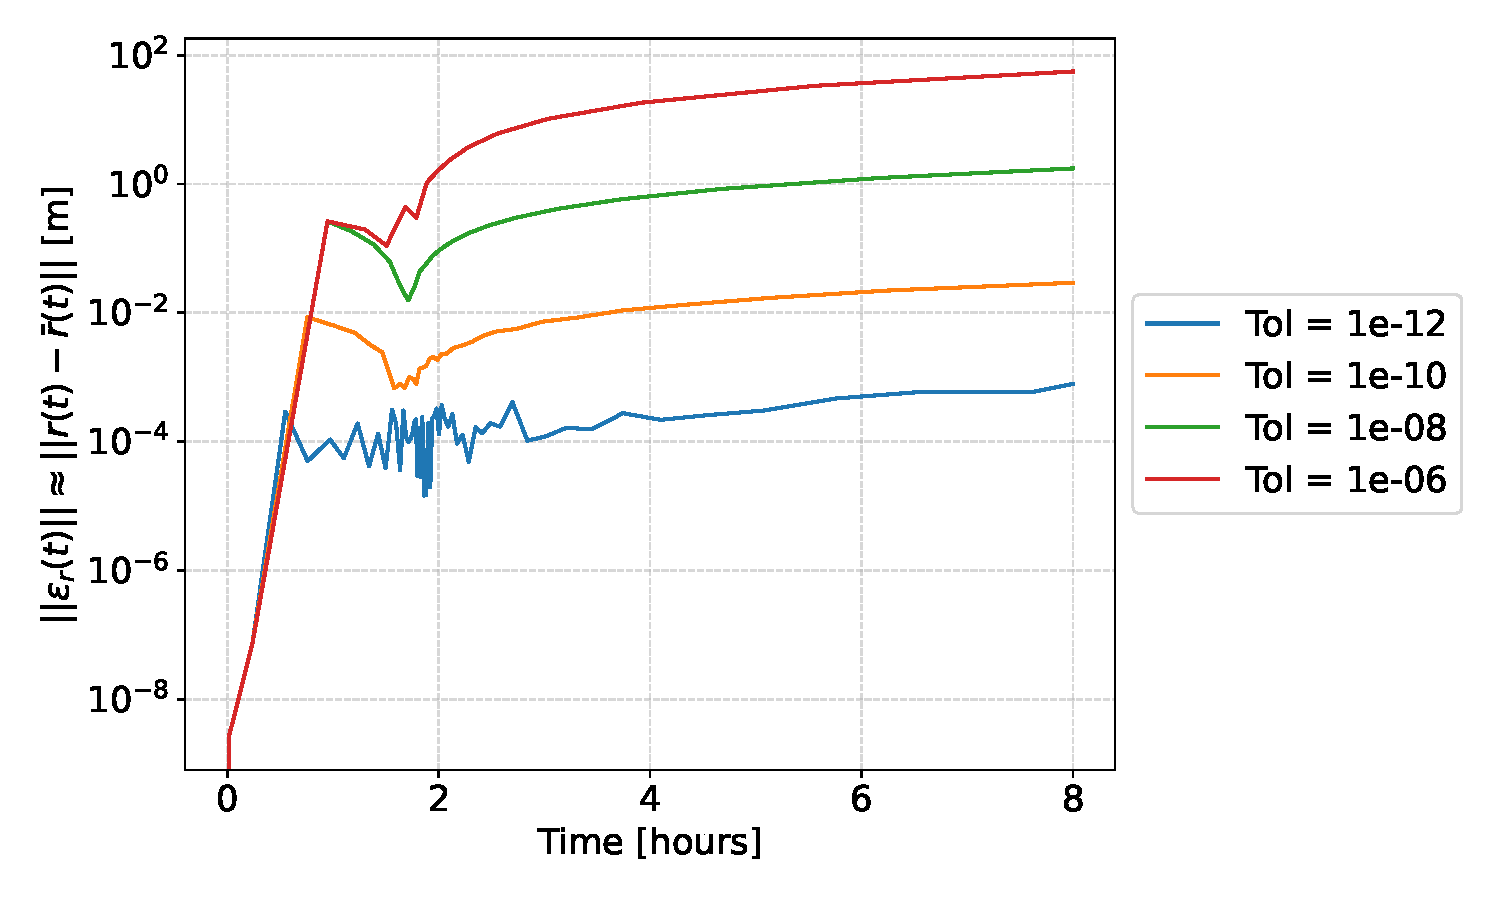
\includegraphics[width=0.7\textwidth]{../../figures/Q3a_error_vs_time_flyby.pdf}
    \caption{Integration error as a function of time for the flyby phase and for different error tolerances.}
    \label{fig:Q3a_error_vs_time_flyby}
\end{figure}

\begin{figure}[H]
    \centering
    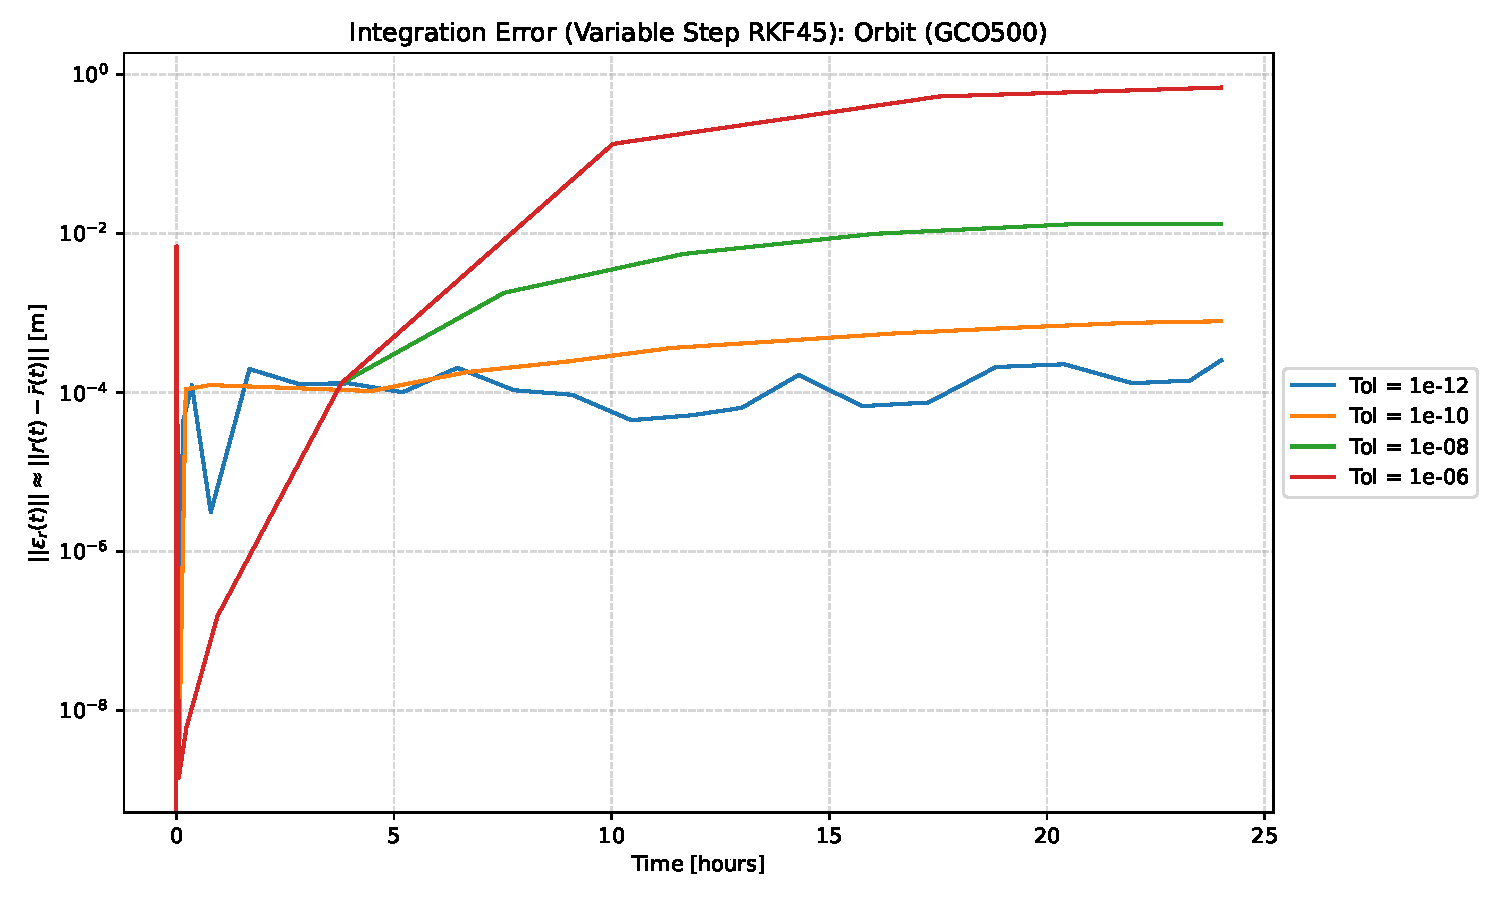
\includegraphics[width=0.7\textwidth]{../../figures/Q3a_error_vs_time_orbit.pdf}
    \caption{Integration error as a function of time for the GCO500 phase and for different error tolerances.}
    \label{fig:Q3a_error_vs_time_orbit}
\end{figure}

Influence of tolerance on observed error:
\begin{itemize}
\item Expected behaviour: smaller tolerance values should yield lower error values. 
\item Observed behaviour: the error values decrease as the tolerance decreases.
% \item Explanation for significant discrepancy (if any): \textbf{\textit{Provide answer}}
\end{itemize}
Visible presence of truncation/rounding error in the figures:
\begin{itemize}
\item Expected behaviour: because the time step control method assumes dominant truncation error, it will reduce the timestep up to a minimum imposed of $10^{-12}$ s if needed, likely incurring in rounding errors. 
\item Observed behaviour: the cases with the smallest tolerances show an error evolution indicative of rounding-driven error. 
% \item Explanation for significant discrepancy (if any): \textbf{\textit{Provide answer}}
\end{itemize}
\subsection*{b}

\begin{figure}[H]
    \centering
    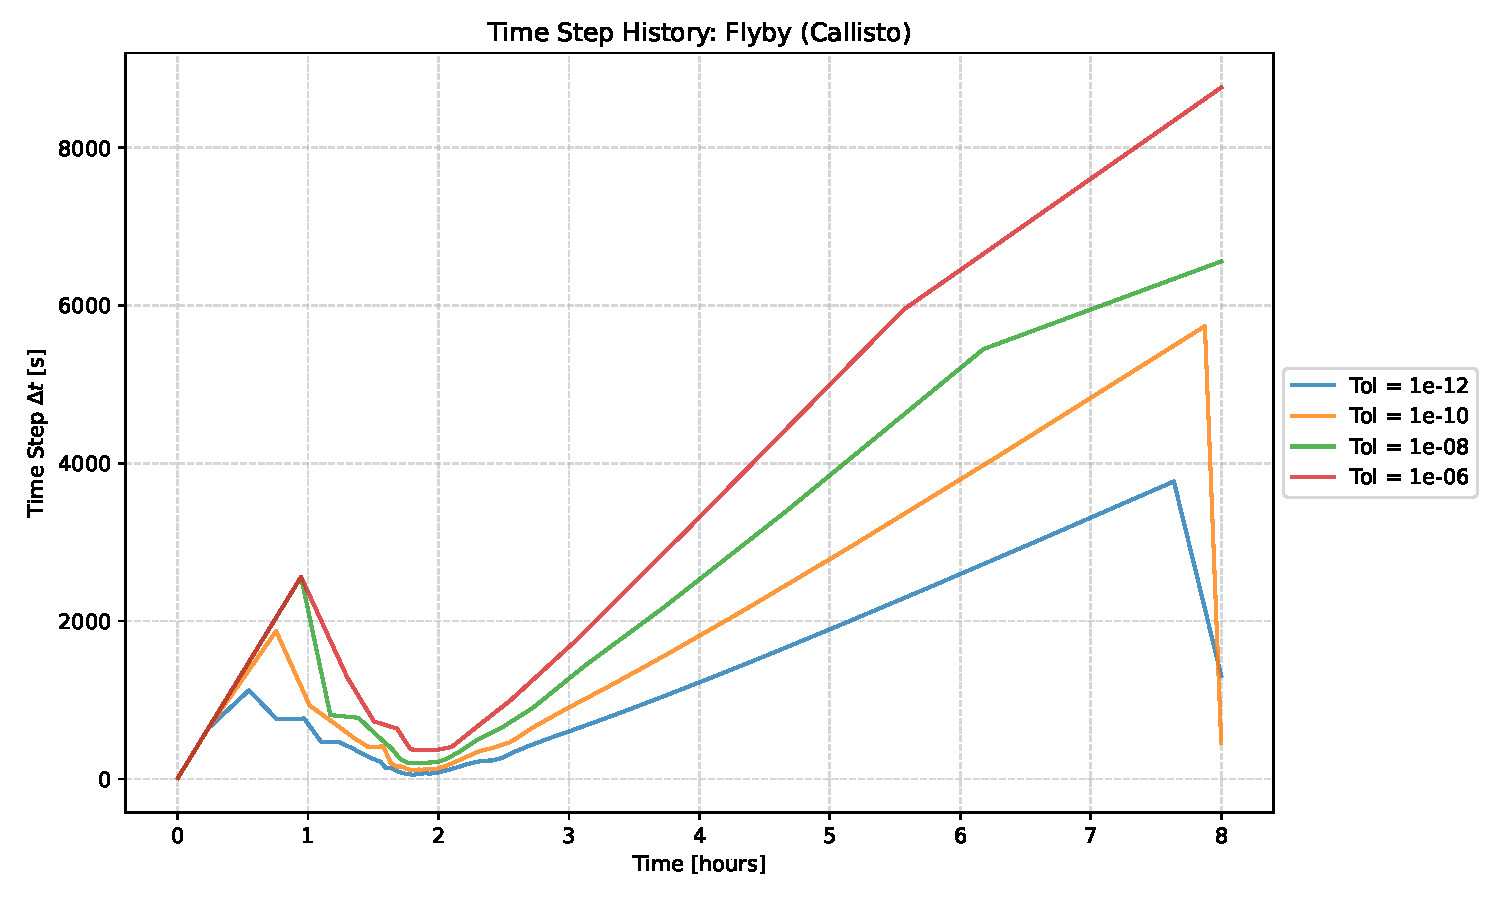
\includegraphics[width=0.7\textwidth]{../../figures/Q3b_timestep_vs_time_flyby.pdf}
    \caption{Time step as a function of time for the flyby phase, for the different tolerances.}
    \label{fig:Q3b_time_step_vs_time_flyby}
\end{figure}

\begin{figure}[H]
    \centering
    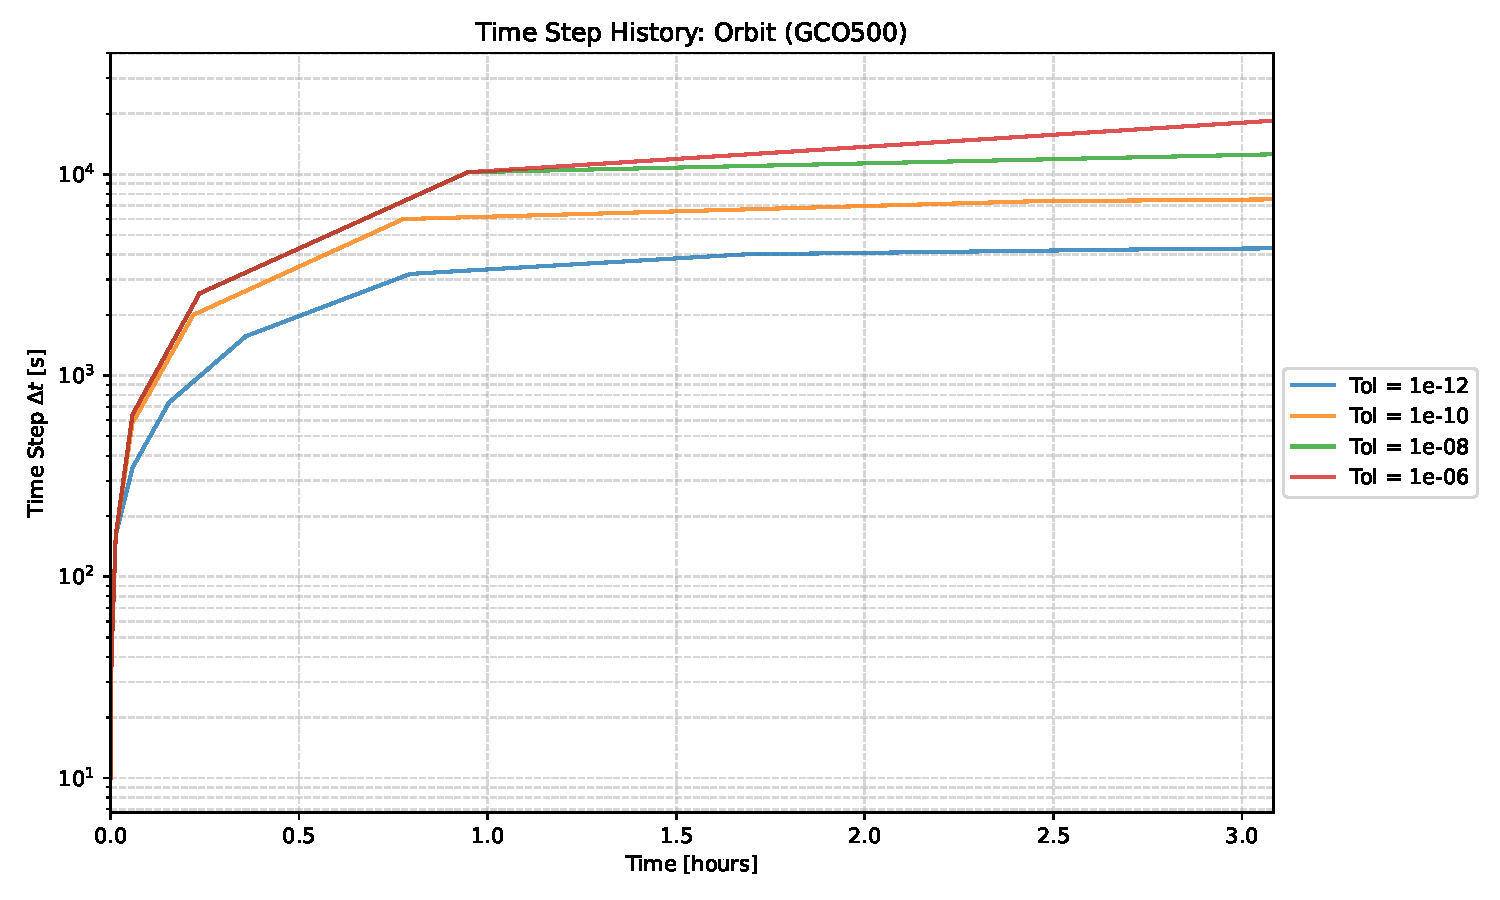
\includegraphics[width=0.7\textwidth]{../../figures/Q3b_timestep_vs_time_orbit.pdf}
    \caption{Time step as a function of time for the GCO500 phase, for the different tolerances.}
    \label{fig:Q3b_time_step_vs_time_orbit}
\end{figure}

\subsection*{c}
% Reason for once-per-orbit trend in time step: \textbf{\textit{Provide answer}}\\
% \\
Reason for sharp decreases in time step: local variations in the acceleration field (faster variations of the dynamics), where the step size control method needs to reduce the time step to keep the error within the specified tolerance.
\subsection*{d}

For propagation using Cartesian state vector, a typical choice is to use a block-wise step size control method, where the state vector is divided into blocks of position and velocity components, and the error is controlled separately for each block.\footnote{\url{https://py.api.tudat.space/en/latest/dynamics/propagation_setup/integrator.html\#tudatpy.dynamics.propagation_setup.integrator.step_size_control_blockwise_scalar_tolerance}}

\begin{lstlisting}
    block_indices = [(0, 0, 3, 1), (3, 0, 3, 1)]
    step_size_control_settings_blockwise = (
        propagation_setup.integrator.step_size_control_blockwise_scalar_tolerance(
            block_indices, current_tolerance, current_tolerance
        )
    )
\end{lstlisting}

\begin{figure}[H]
    \centering
    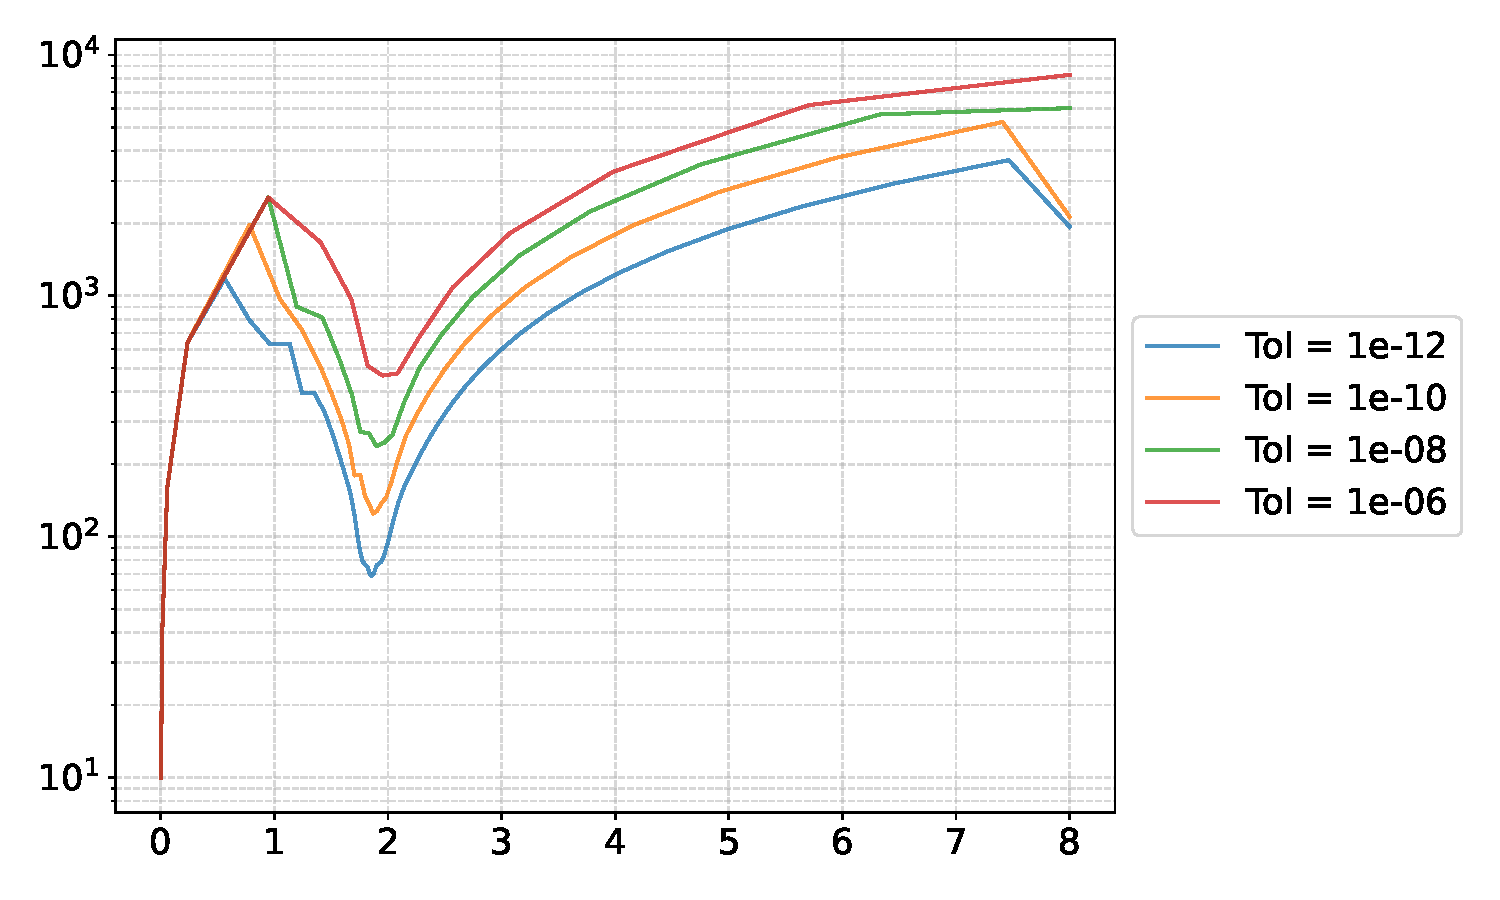
\includegraphics[width=0.7\textwidth]{../../figures/Q3d_blockwise_timestep_vs_time_flyby.pdf}
    \caption{Time step as a function of time for the flyby phase, for the different tolerances, with block-wise step size control.}
    \label{fig:Q3d_blockwise_timestep_vs_time_flyby}
\end{figure}

\begin{figure}[H]
    \centering
    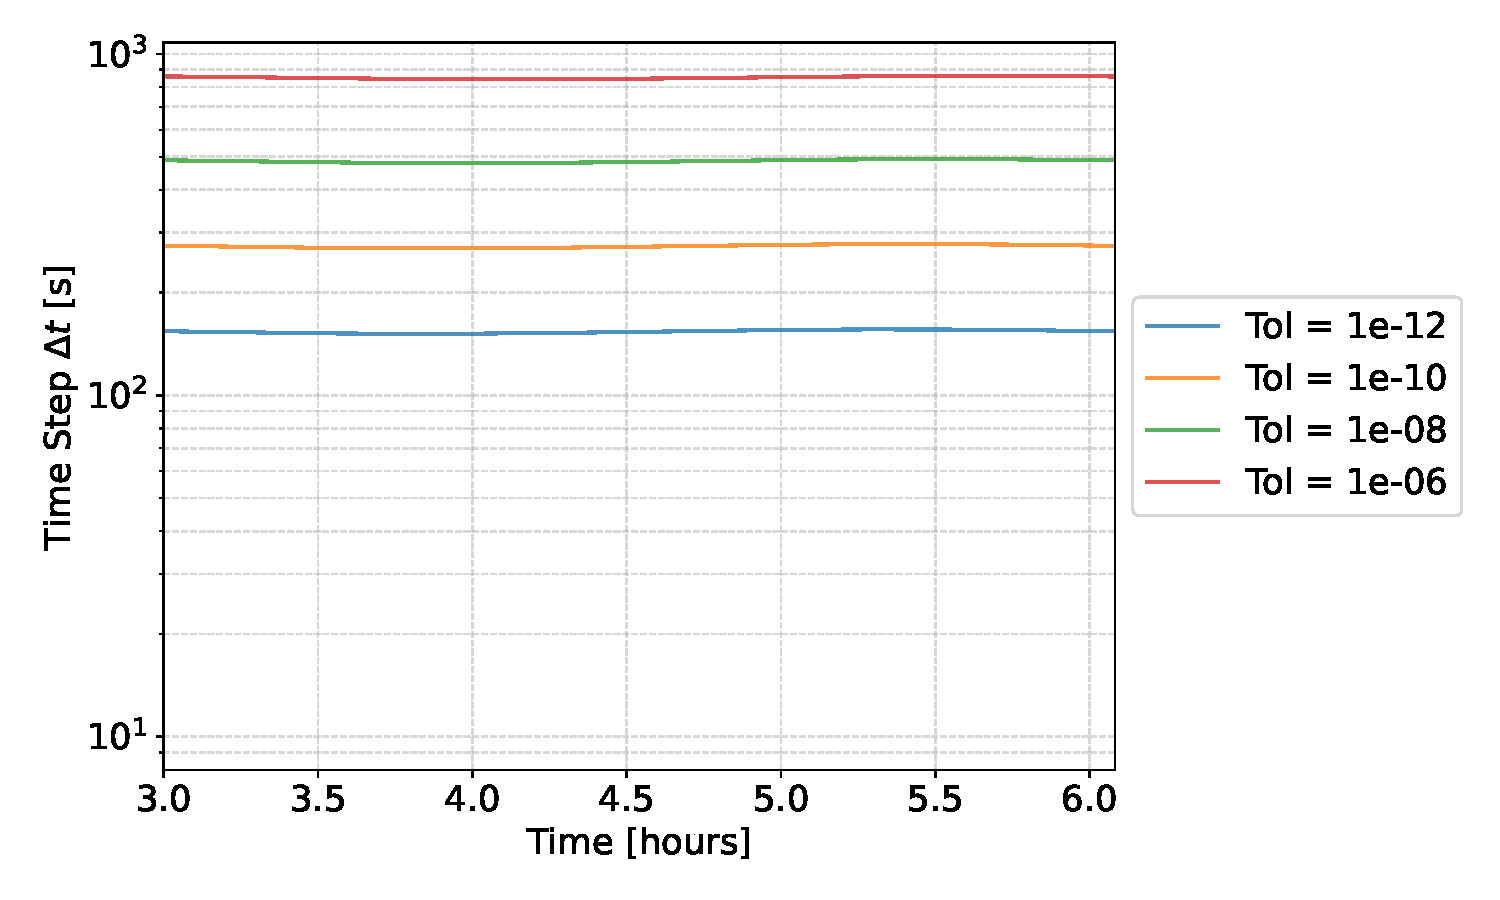
\includegraphics[width=0.7\textwidth]{../../figures/Q3d_blockwise_timestep_vs_time_orbit.pdf}
    \caption{Time step as a function of time for the GCO500 phase, for the different tolerances, with block-wise step size control.}
    \label{fig:Q3d_blockwise_timestep_vs_time_orbit}
\end{figure}

\clearpage
\section*{Question 4}
\subsection*{a}

\begin{figure}[H]
    \centering
    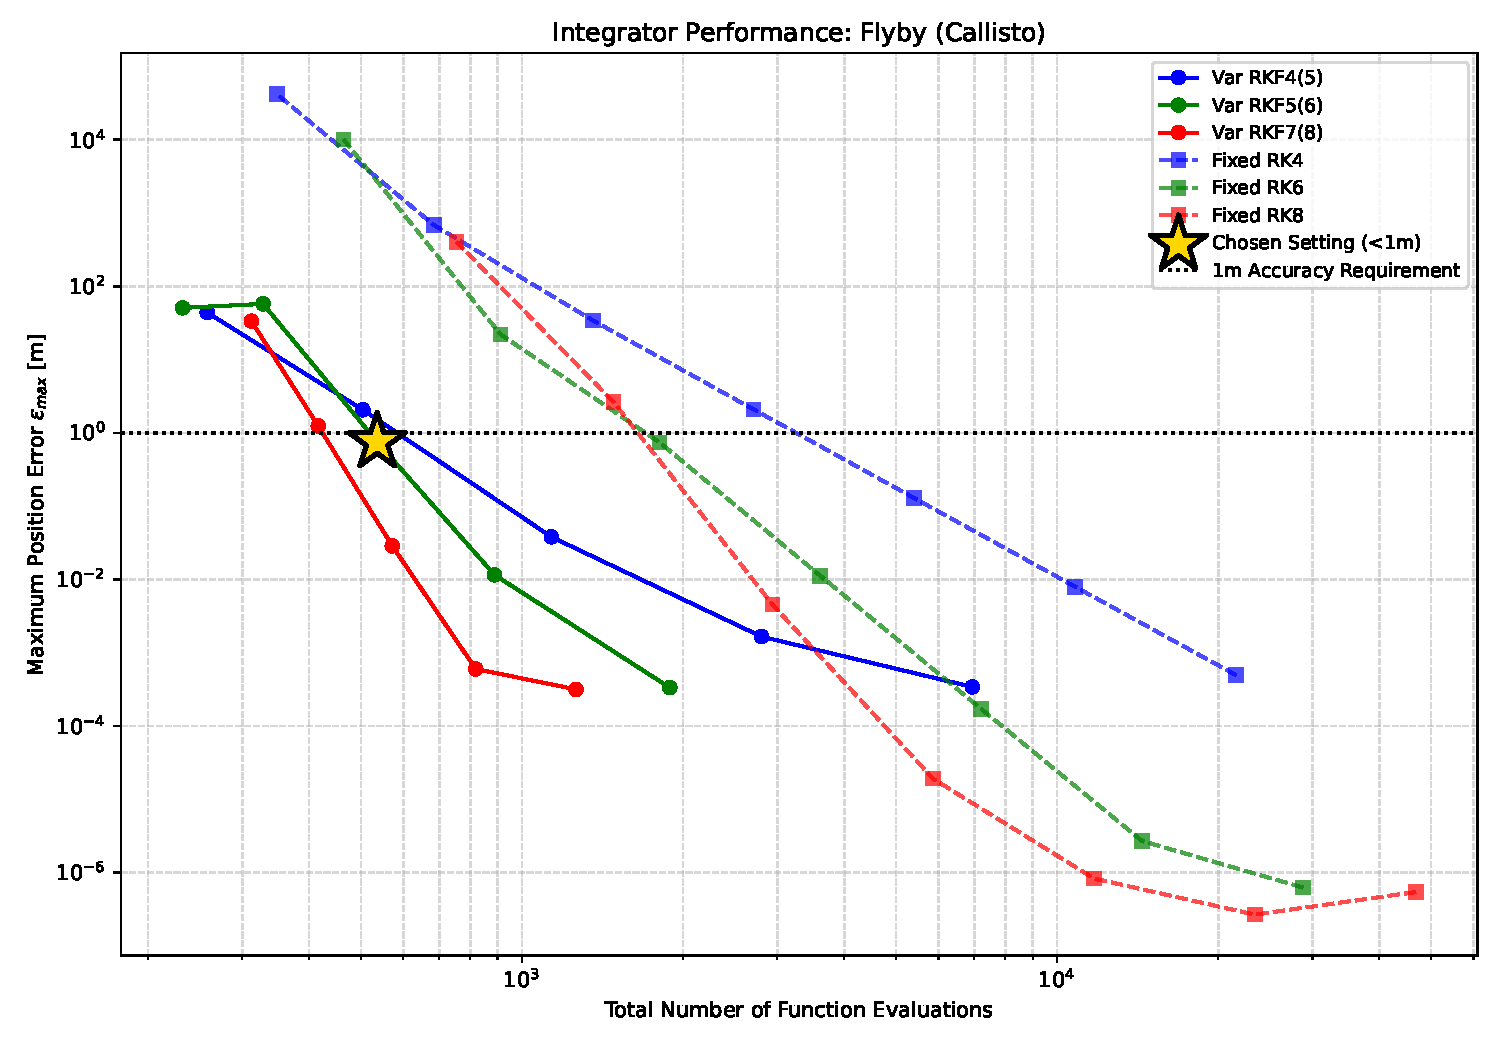
\includegraphics[width=0.7\textwidth]{../../figures/Q4a_workload_diagram_flyby.pdf}
    \caption{Number of function evaluations versus maximum error for the flyby phase, for the different integrators.}
    \label{fig:Q4a_workload_diagram_flyby}
\end{figure}

\begin{figure}[H]
    \centering
    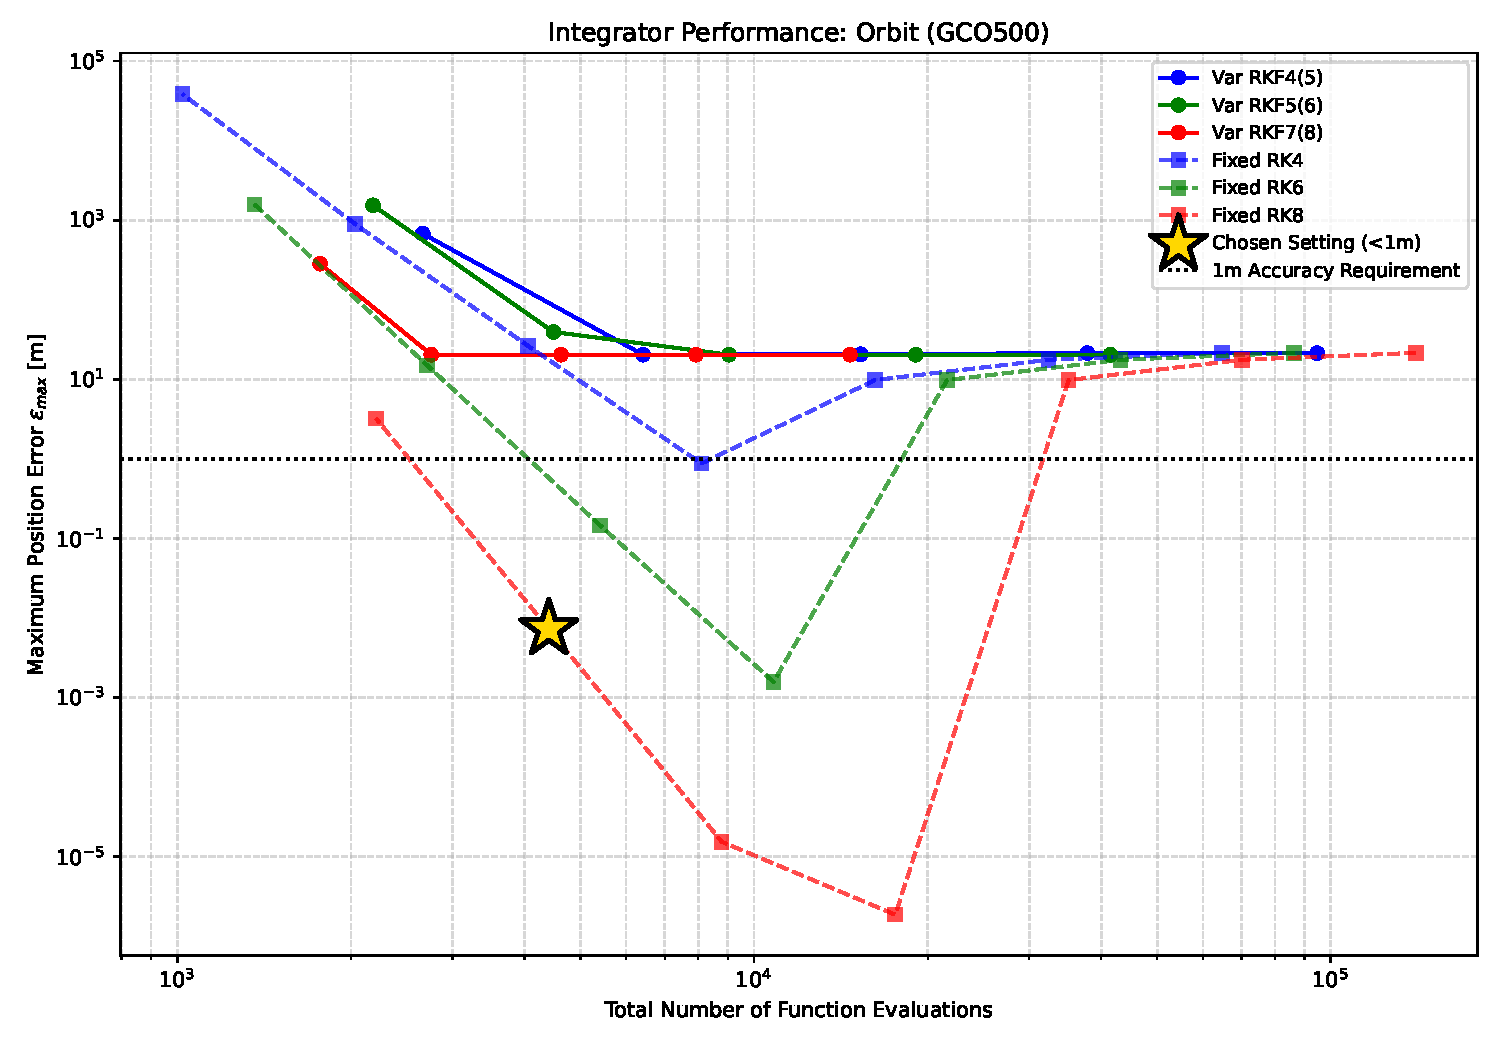
\includegraphics[width=0.7\textwidth]{../../figures/Q4a_workload_diagram_orbit.pdf}
    \caption{Number of function evaluations versus maximum error for the GCO500 phase, for the different integrators.}
    \label{fig:Q4a_workload_diagram_orbit}
\end{figure}

\subsection*{b}

The chosen integrators are indicated in \autoref{fig:Q4b_chosen_error_vs_time_flyby} and \autoref{fig:Q4b_chosen_error_vs_time_orbit} by a star marker.

Integrator choice for orbit phase: RK8 with fixed step size of 256 s.

Integrator choice for flyby phase: RKF5(6) with tolerance of $10^{-10}$.

Reasons for your integrator choices: the chosen integrators are the ones with the lowest number of function evaluations for the position accuracy requirement of 1 m. 

\begin{figure}[H]
    \centering
    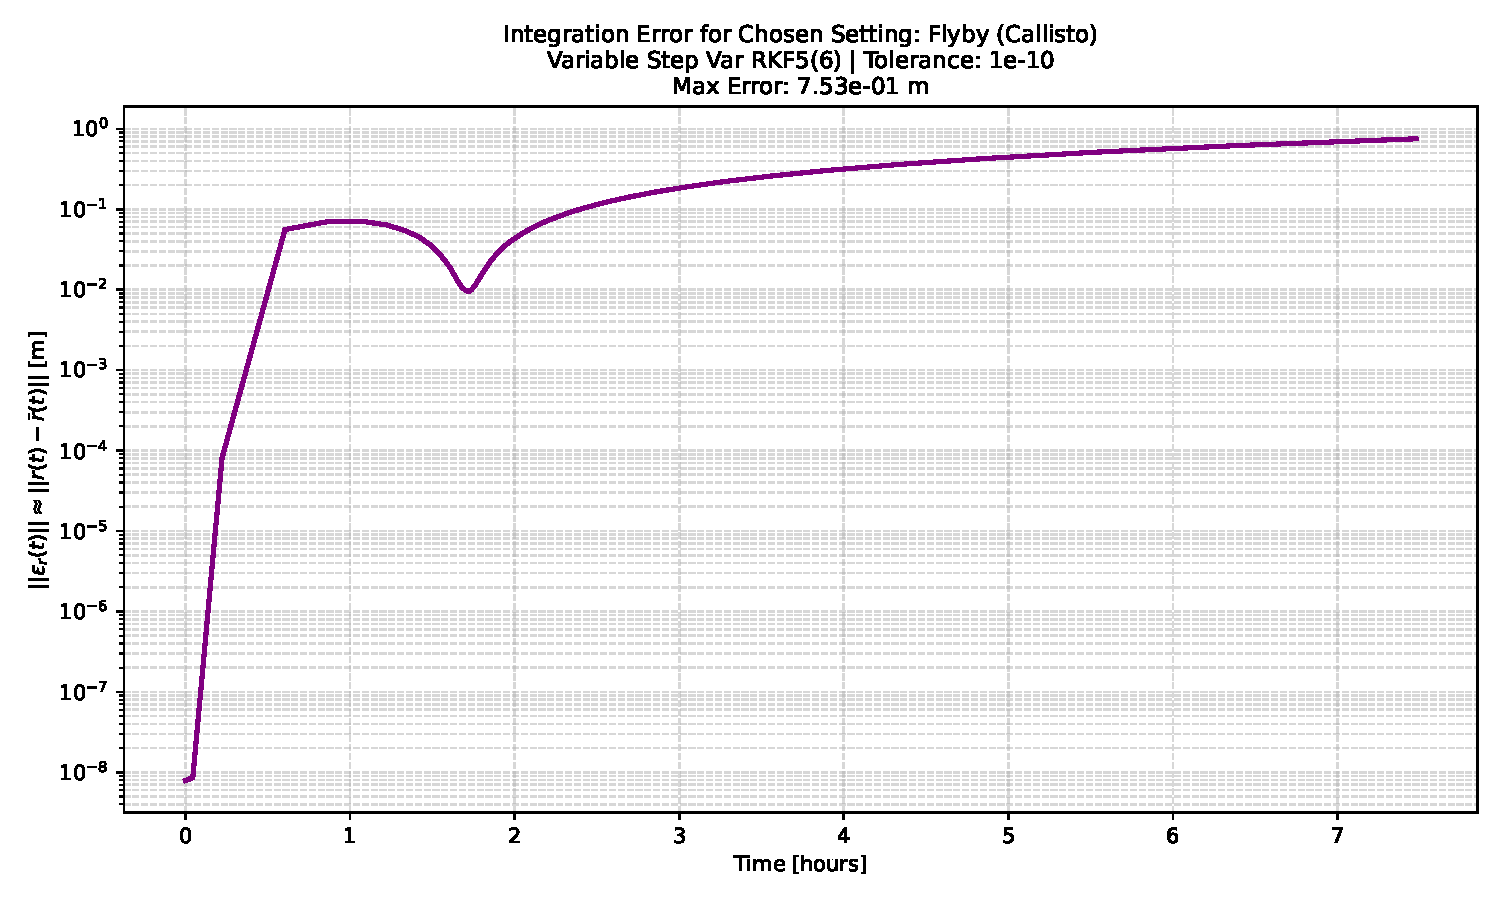
\includegraphics[width=0.7\textwidth]{../../figures/Q4b_chosen_error_vs_time_flyby.pdf}
    \caption{Number of function evaluations versus maximum error for the flyby phase, for the different integrators.}
    \label{fig:Q4b_chosen_error_vs_time_flyby}
\end{figure}

\begin{figure}[H]
    \centering
    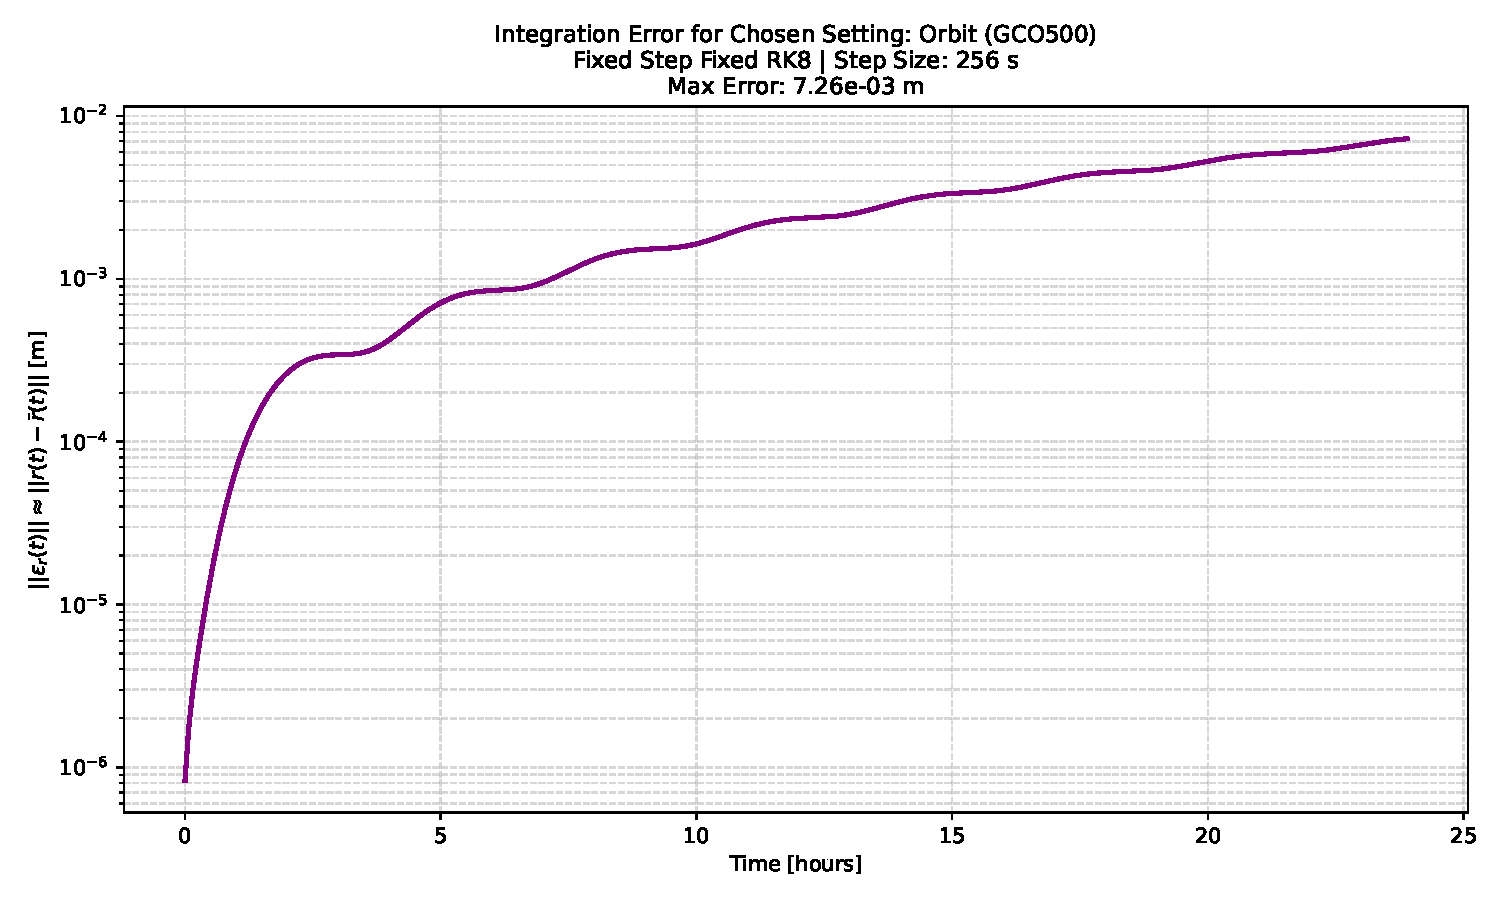
\includegraphics[width=0.7\textwidth]{../../figures/Q4b_chosen_error_vs_time_orbit.pdf}
    \caption{Number of function evaluations versus maximum error for the GCO500 phase, for the different integrators.}
    \label{fig:Q4b_chosen_error_vs_time_orbit}
\end{figure}

\clearpage
\section*{Question 5}
\subsection*{a}

\begin{figure}[H]
    \centering
    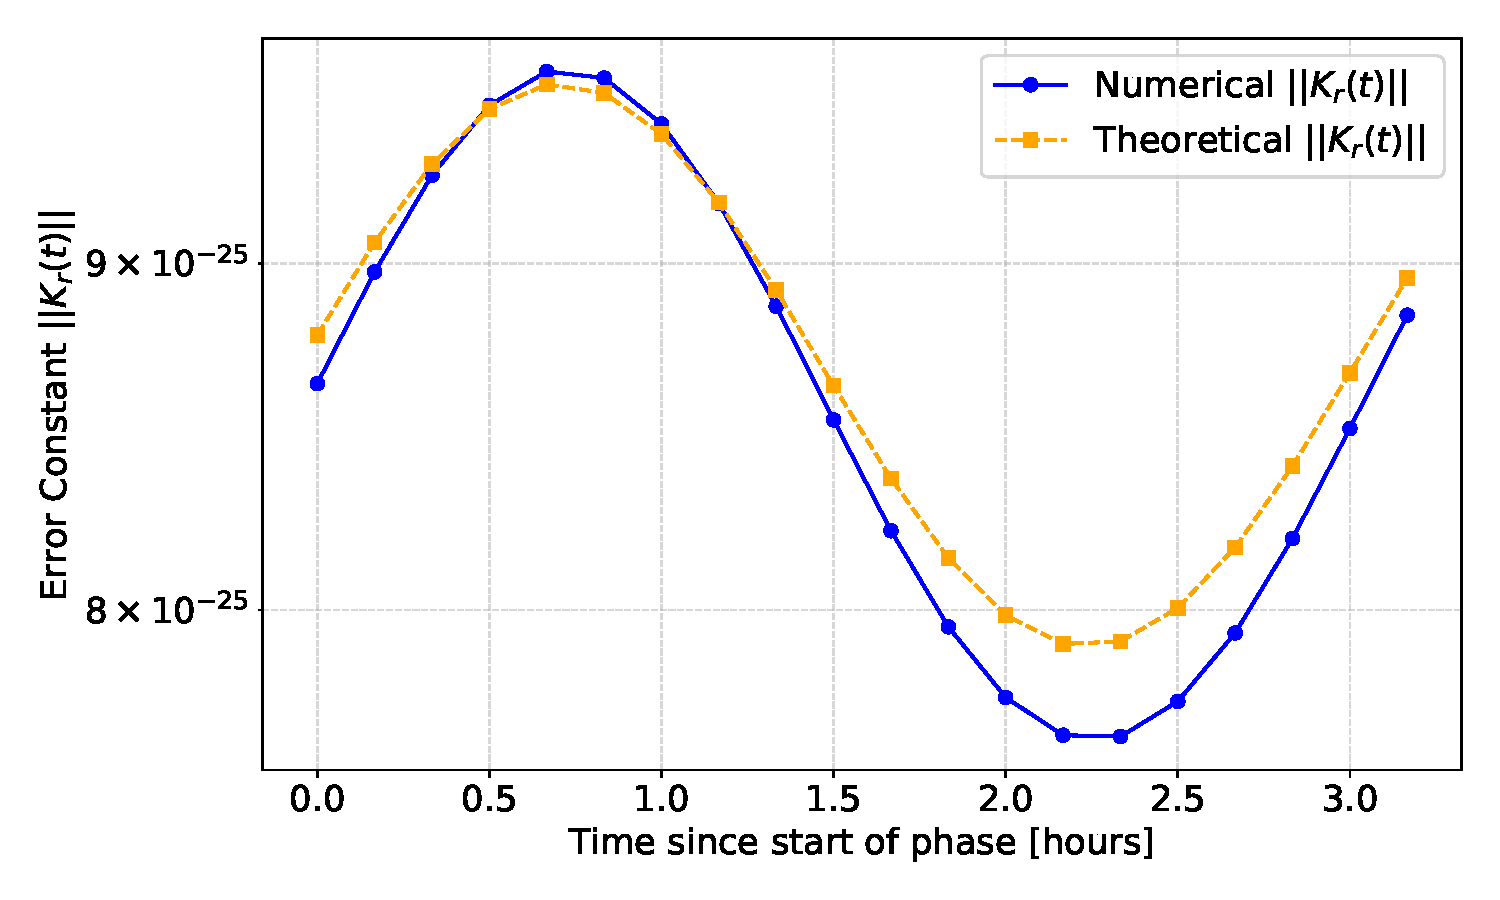
\includegraphics[width=0.7\textwidth]{../../figures/Q5_Kr_RKF78.pdf}
    \caption{Condition numbers for the RKF7(8) fixed step integrator, for the conditions described in the assignment.}
    \label{fig:Q5_Kr_RKF78}
\end{figure}

\subsection*{b}

The Cartesian position, assuming circular motion in XY plane, can be expressed as:

\begin{equation}
    \mathbf{r}(t) = \begin{bmatrix}r(\tilde{t_0}) \cos{(n t)} \\ r(\tilde{t_0}) \sin{(n t)} \\ 0\end{bmatrix},
\end{equation}
where $n$ is the mean motion, and $r(\tilde{t_0})$ is the radius at the initial time $\tilde{t_0}$.

Thus, the 8th derivative of the position can be expressed as:

\begin{equation}
    \frac{\mathrm{d}^8 \mathbf{r}(t)}{\mathrm{d}t^8} = r(\tilde{t_0}) n^8 \begin{bmatrix} \cos{(n t)} \\ \sin{(n t)} \\ 0\end{bmatrix} \Rightarrow ||\frac{\mathrm{d}^8 \mathbf{r}(t)}{\mathrm{d}t^8}|| = r(\tilde{t_0}) n^8,
\end{equation}

Also, the Taylor expansion around $\tilde{t_0}$ of the position up to 8th order can be expressed as:

\begin{equation}
    \mathbf{r}(\tilde{t_0} + \Delta t) = \sum_{k=0}^8 \frac{1}{k!} \frac{\mathrm{d}^k \mathbf{r}(t)}{\mathrm{d}t^k} (\Delta t)^k + \mathcal{O}((\Delta t)^9),
\end{equation}

So, since the RK7 method can be approximated by the Taylor expansion up to 7th order \cite{hernandez2020interpolacion}, the local truncation error can be expressed as:

\begin{equation}
    \epsilon(t) = \mathbf{r}(\tilde{t_0} + \Delta t) - \sum_{k=0}^7 \frac{1}{k!} \frac{\mathrm{d}^k \mathbf{r}(t)}{\mathrm{d}t^k} (\Delta t)^k = \frac{1}{8!} \frac{\mathrm{d}^8 \mathbf{r}(t)}{\mathrm{d}t^8} (\Delta t)^8 + \mathcal{O}((\Delta t)^9) \Rightarrow ||\epsilon(t)|| \approx \frac{1}{8!} ||\frac{\mathrm{d}^8 \mathbf{r}(t)}{\mathrm{d}t^8}|| (\Delta t)^8,
\end{equation}

\begin{equation} \label{eq:kr_rk7}
||\mathbf{K}_{\mathbf{r}}(t)|| = \frac{r(\tilde{t_0}) n^8}{8!}.
\end{equation}

The plot for the analytical $||\mathbf{K}_{\mathbf{r}}(t)||$ is also included in \autoref{fig:Q5_Kr_RKF78}.

\subsection*{c}

Following the same reasoning as in question (b), the second derivative of the position can be expressed as:
\begin{equation}
    \frac{\mathrm{d}^2 \mathbf{r}(t)}{\mathrm{d}t^2} = - r(\tilde{t_0}) n^2 \begin{bmatrix} \cos{(n t)} \\ \sin{(n t)} \\ 0\end{bmatrix} \Rightarrow ||\frac{\mathrm{d}^2 \mathbf{r}(t)}{\mathrm{d}t^2}|| = r(\tilde{t_0}) n^2,
\end{equation}

and the Taylor expansion around $\tilde{t_0}$ of the position up to 2nd order can be expressed as:

\begin{equation}
    \epsilon(t) = \mathbf{r}(\tilde{t_0} + \Delta t) - \sum_{k=0}^1 \frac{1}{k!} \frac{\mathrm{d}^k \mathbf{r}(t)}{\mathrm{d}t^k} (\Delta t)^k = \frac{1}{2!} \frac{\mathrm{d}^2 \mathbf{r}(t)}{\mathrm{d}t^2} (\Delta t)^2 + \mathcal{O}((\Delta t)^3) \Rightarrow ||\epsilon(t)|| \approx \frac{1}{2!} ||\frac{\mathrm{d}^2 \mathbf{r}(t)}{\mathrm{d}t^2}|| (\Delta t)^2,
\end{equation}

\begin{equation} \label{eq:kr_euler}
||\mathbf{K}_{\mathbf{r}}(t)||= \frac{r(\tilde{t_0}) n^2}{2!}. 
\end{equation}

\begin{figure}[H]
    \centering
    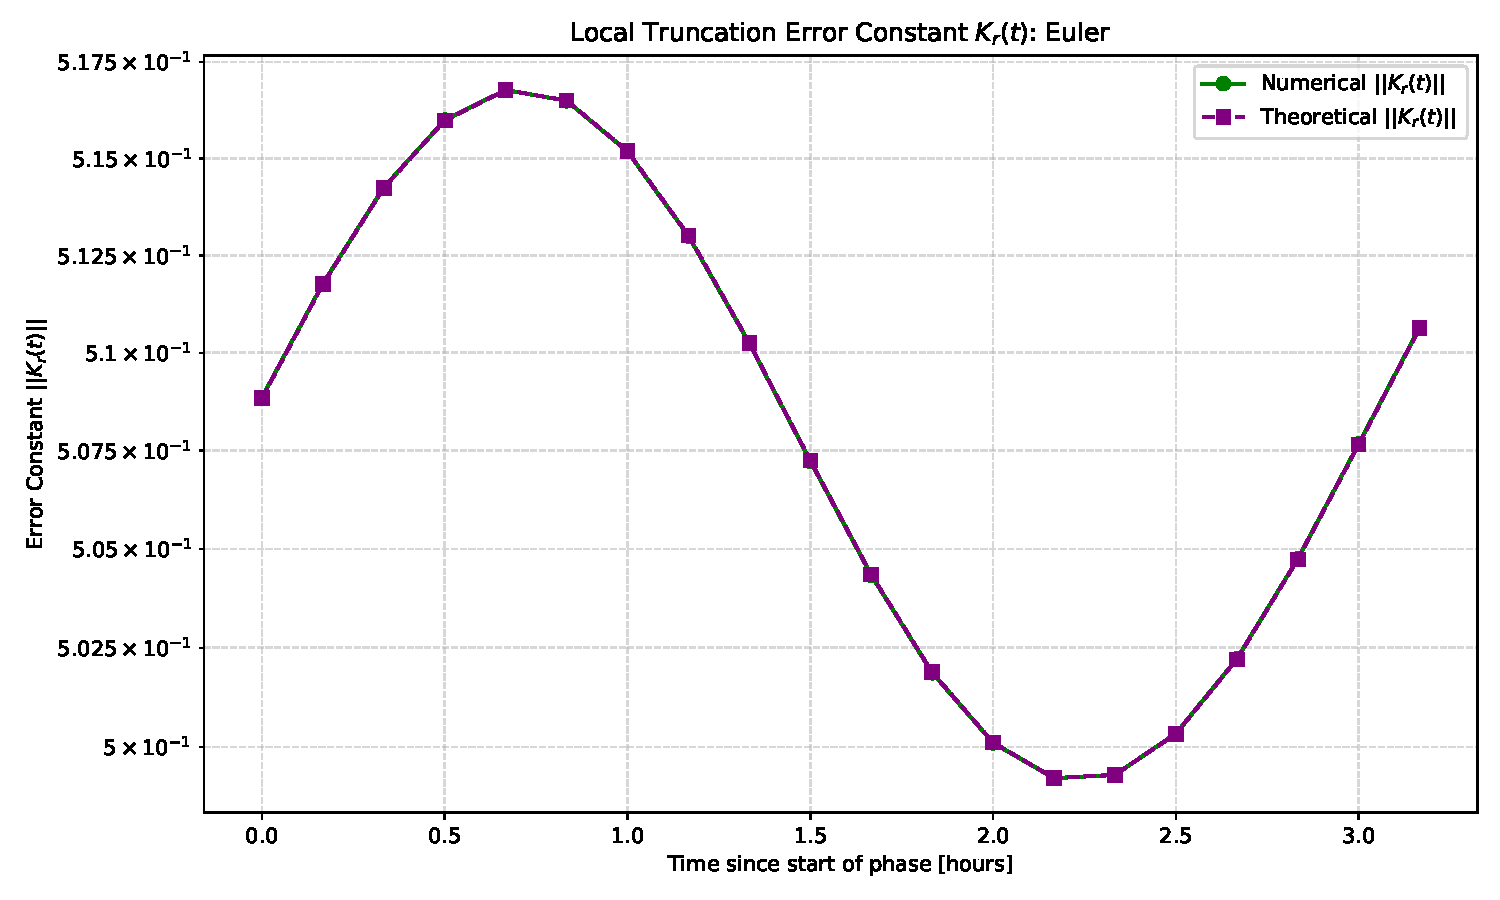
\includegraphics[width=0.7\textwidth]{../../figures/Q5_Kr_Euler.pdf}
    \caption{Condition numbers for the Euler fixed step integrator, for the conditions described in the assignment.}
    \label{fig:Q5_Kr_Euler}
\end{figure}\subsection*{d}

% \textit{\textbf{Provide reasons for difference in validity of analytical result for Euler and RKF results}}\\

First, it has to be noted that the analytical condition number calculated is much more similar to the one obtained for the Euler method compared with the RKF7(8) method, as it can be observed in \autoref{fig:Q5_Relative_Error_Comparison}.

The main reason for the difference in the approximation between the Euler and RKF7(8) methods is that the condition number is calculated with an approximation of the mean motion $n$ under the assumptions listed. 
Since $|\mathbf{K}_{\mathbf{r}}(t)||$ is proportional to $n^{p+1}$, where $p$ is the order of the method, any error in the estimation of $n$ will be amplified by a factor of $p+1$ in the condition number, which leads to a the bigger error observed for the higher-order method.

\begin{figure}[H]
    \centering
    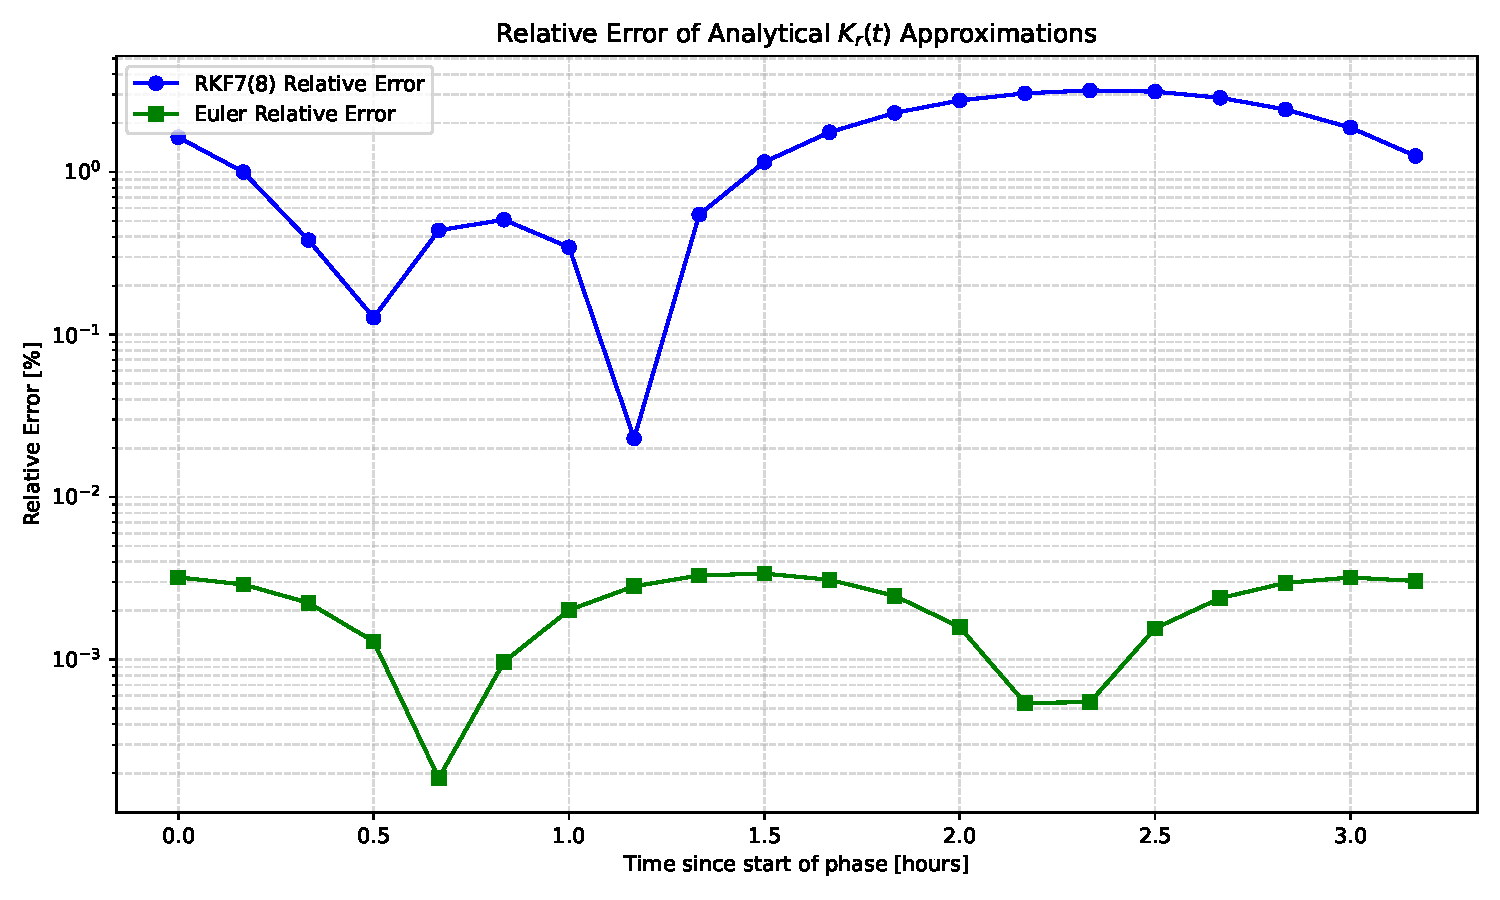
\includegraphics[width=0.7\textwidth]{../../figures/Q5_Relative_Error_Comparison.pdf}
    \caption{Relative errors in the condition numbers for the RKF7(8) and Euler fixed step integrators, for the conditions described in the assignment.}
    \label{fig:Q5_Relative_Error_Comparison}
\end{figure}

\clearpage
\bibliographystyle{plain}
\bibliography{references}

\end{document}
